\documentclass[a4paper,12pt]{report}
\usepackage[a4paper,inner = 0.5cm, outer = 0.5cm, top = 2cm, bottom = 2cm]{geometry}

\usepackage[english,romanian]{babel}
\usepackage{blindtext}
\usepackage{fancyhdr}
\usepackage{wrapfig}
\usepackage{graphicx}
\usepackage{amsmath}
\usepackage{caption}
\usepackage{dirtytalk}
\usepackage{url}
\usepackage{listings}

\renewenvironment{abstract}[1]
  {\bigskip\selectlanguage{#1}%
   \begin{center}\bfseries\abstractname\end{center}}
  {\par\bigskip}

\newcommand{\source}[1]{\caption*{Sursă: {#1}} }

\fancyhf{}
\renewcommand{\headrulewidth}{2pt}
\renewcommand{\footrulewidth}{1pt}
\fancyhead[LE]{\leftmark}
\fancyhead[RO]{\rightmark}
\linespread{1.25}
\hyphenpenalty=50000
\begin{document}
\begin{titlepage}
    \begin{center}
        \begin{figure}[htbp]
            \centering
            \begin{minipage}{0.2\textwidth}
              
\includegraphics[width=\linewidth]{images/poza_stanga.png}
            \end{minipage}\
            \begin{minipage}{0.5\textwidth}
                \begin{large}
                    \textbf{UNIVERSITATEA DIN BUCUREȘTI}\\
                    \\
                    \begin{center}
                    \textbf{FACULTATEA\\
                                DE\\
                    MATEMATICĂ ȘI INFORMATICĂ}
								\end{center}
                \end{large}
            \end{minipage}
            \begin{minipage}{0.2\textwidth}
              
\includegraphics[width=\linewidth]{images/poza_dreapta.png}
            \end{minipage}
        \end{figure}
        
        \vspace*{1cm}
        
        \begin{large}
            \textbf{SPECIALIZAREA INFORMATICĂ}
        \end{large}

        \vspace{2.5cm}
        \begin{LARGE}
            \textbf{LUCRARE DE DISERTAŢIE}\\
            \vspace*{0.5cm}
            \textbf{EXECUŢIA WORKFLOW-URILOR DURABILE ÎN CLOUD}
        \end{LARGE}
            
        \vspace{2.5cm}
        \begin{large}
            \textbf{Absolvent}\\
            \vspace*{0.25cm}
            \textbf{Moldovan George-Alexandru}
        \end{large}
        
        \vspace{2cm}
        \begin{large}
            \textbf{Coordonator științific}\\
            \vspace*{0.25cm}
            \textbf{Prof. dr. Letiţia Marin}
        \end{large}
        
        \vspace{2.5cm}
        \begin{large}
            \textbf{București, septembrie 2022}
        \end{large}
    \end{center}
\end{titlepage}
\newgeometry{a4paper,inner = 1.7cm, outer = 2.7cm, top = 2cm, bottom = 2cm, bindingoffset = 1.2cm}
\begin{abstract}{romanian}
\par Considerând trend-ul ascendent al arhitecturii orientate spre microservicii si migrarea de la vechiul mod de dezvoltare monolit, aceasta lucrare de disertaţie işi propune analiza soluţiilor prezente in piaţa în ceea ce priveşte managementul unei arhitecturi pe microservicii în cloud, şi analiza unor contribuţii personale aduse unui framework open-source de gestionare a workflow-urilor în cloud. Sistemele informatice preiau din complexitatea operaţiilor de zi cu zi, astfel că arborii de decizie trebuie interpretaţi şi gestionaţi în mod corect pentru a realiza un sistem care sa indeplinească cerinţele de piaţă curente. Pentru o lunga perioadă de timp, problema gestionării tranzacţiilor distribuite si management-ul workflow-urilor a fost inexistentă, deoarece într-un sistem monolit, caracteristicile tranzacţionale ale bazelor de date ce susţineau astfel de sisteme erau indeajuns pentru a avea toate garanţiile necesare astfel încât sistemul sa fie mereu lăsat într-o stare consistentă. Microserviciile şi arhitecturile distribuite in general, deşi vin cu o serie lunga de avantaje, poate cel mai greu de gestionat lucru este management-ul stării unei acţiuni, atunci cand aceasta se întinde pe mai multe microservicii, şi pe o durată lungă de timp. 
\end{abstract}
\begin{abstract}{english}\par Considering the upward trend of microservices-oriented architecture and the migration from the old monolithic development mode, this dissertation aims to analyze the solutions present in the market in terms of managing a microservices architecture in the cloud, and the analysis of personal contributions to a open-source framework for managing cloud workflows. Information systems take over the complexity of day-to-day operations, so decision trees must be interpreted and managed correctly to achieve a system that meets current market requirements. For a long time, the problem of distributed transaction management and workflow management was non-existent, because in a monolithic system, the transactional characteristics of the databases that supported such systems were sufficient to have all the necessary guarantees so that the system should always be left in a consistent state. Distributed microservices and architectures in general, although they come with a long list of advantages, perhaps the most difficult thing to manage is the management of the state of an action, when it extends over several microservices, and over a long period of time.
\end{abstract}
\tableofcontents
\pagenumbering{arabic}
\setcounter{page}{2}
\chapter{Introducere}
\section{Motivatie}
\quad Unul din principiile de baza ale programării este reutilizarea. Motivaţia din spatele acestei lucrări o reprezintă dorinţa de o contribui la un framework care rezolvă o problemă generică, cu care se confruntă toţi dezvoltatorii care trebuie sa gestioneze tranzacţii distribuite. Analiza diferitelor metode pentru rezolvarea problemei de gestiune a workflow-urilor în cloud, în special într-o arhitectură ce se bazează pe funcţii în cloud a fost o prioritate pentru mine în ultimii ani. 
\par
Serverless, sau Functions-as-a-Service (FaaS), este o paradigmă din ce în ce mai populară pentru dezvoltarea de aplicații, deoarece oferă scalare infintă implicită și facturare bazată pe consum. Cu toate acestea, garanţiile slable de execuţie și suportul nativ pentru stocare a stării a FaaS creează provocări serioase atunci când se dezvoltă aplicații care necesită stare persistentă, garanţii de execuţie sau sincronizare. Acest lucru a motivat o nouă generație de soluţii serverless care oferă abstractizări ce stochează starea aplicaţiei. De exemplu, noua soluţie Azure Durable Functions (DF), o extindere peste deja existenta Azure Functions. Modelul îmbunătățește FaaS cu actori, fluxuri de lucru și secțiuni critice.
\par
În acest context în care dezvoltatorii incearcă sa dezvolte aplicaţii ce gestiunează workflow-uri  de lungă durată, cu toţii rezolvă aceeaşi problemă şi anume lipsa separării intre nivelul de execuţie si nivelul de stocare a soluţiilor existente FaaS. Cu toţii rezolvă o problemă generică, de salvare a stării în anumite puncte ale execuţiei, pentru a putea relua workflow-ul în eventualitatea în care agentul pe care rulează aplicaţie pică inainte de finalizarea workflow-ului. Acest lucru era foarte greu de realizat in arhitecturi serverless deoarece toate soluţiile existente până la apariţia Azure Durable Functions, suportau doar execuţii stateless în mod standard. Deci până la apariţia soluţiilor ce oferă garanţii de execuţie puternice in lumea Serverless, această tehnologie nu era o opţiune populară pentru dezvoltarea aplicaţiilor ce aveau nevoie de gestionare a stării şi era limitată la execuţia unor parţi mici ale aplicaţiilor pentru care starile intermediare nu erau importante. 
\section{Context}
\quad Serverless diferă de conceptele tradiționale de cloud computing în sensul că infrastructura și platformele în care serviciile rulează sunt ascunse clienților. În această abordare, clienții sunt preocupați doar de funcționalitatea dorită a aplicației lor, iar restul este delegată furnizorului de servicii. \par

Scopul serviciilor Serverless este triplu : 
\begin{itemize}
\item Scuteşte dezvoltatorii de servicii cloud de la interacţiunea cu infrastructura sau diferite platforme
\item Converteste modelul de facturare din cel clasic la cel bazat pe consum
\item Scalarea automată a serviciului în funcție de cererea clienților.
\end{itemize}
\par

\begin{wrapfigure}{r}{0.45\textwidth}
	  \begin{center}
        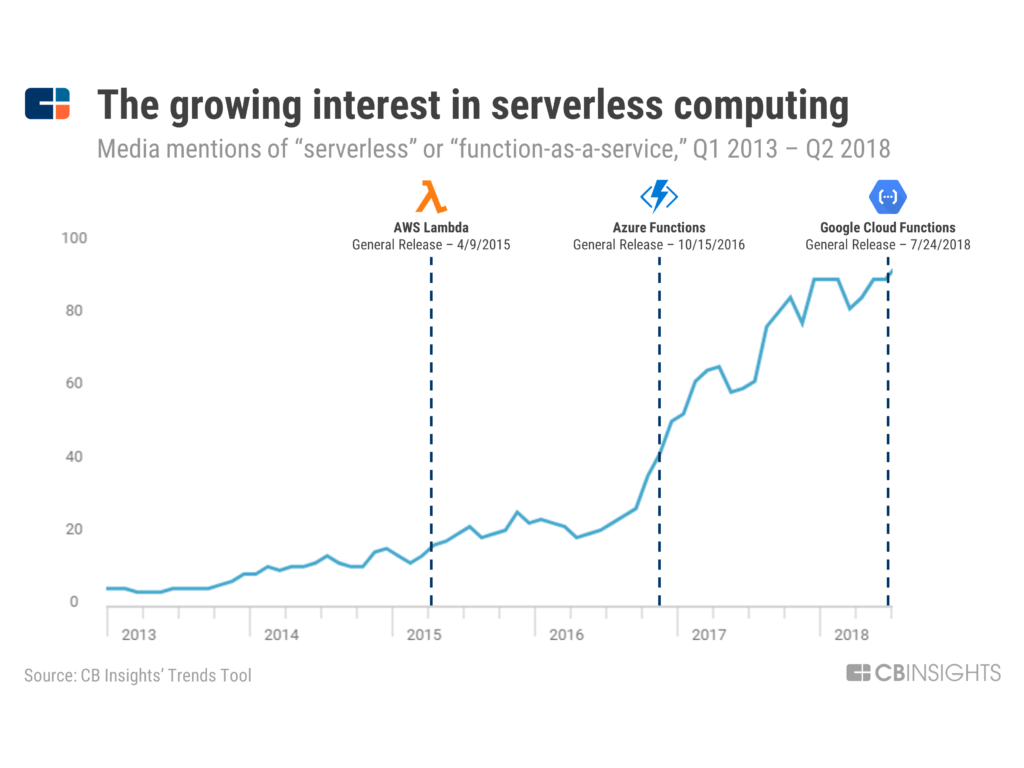
\includegraphics[width=0.4\textwidth]{images/grafic_serverless_computing}
       \caption{Statistică ce evidenţiază importanţa domeniului cloud computing în ultimii ani}
			\label{fig:cloud_computing_graph}
       \source {https://www.cbinsights.com}
    \end{center}
\end{wrapfigure}
Ca rezultat, într-o aplicație cu adevărat Serverless, infrastructura de execuție este ascunsă clientului, iar clientul plătește doar pentru resursele pe care le utilizează efectiv. Serviciul este conceput astfel încât să poată gestiona rapid creșterile de consum prin scalare automată. Entitățile de bază în calculul fără server sunt funcții. Clientul își înregistrează funcțiile în furnizorul de servicii. Apoi, acele funcții pot fi invocate fie de un eveniment, fie direct prin apelarea acestora la cererea utilizatorilor. Rezultatele execuției sunt trimise înapoi clientului. Invocarea funcțiilor este delegată unuia dintre nodurile de calcul disponibile în interiorul furnizorului de servicii. De obicei, aceste noduri sunt containere cloud, cum ar fi Docker [100] sau un mediu de rulare izolat [67].

\par
Deși conceptul de Serverless este relativ nou, acesta și-a deschis drumul în multe aplicații din lumea reală, de la instrumente de colaborare online la sisteme integrate (IoT), având o creştere în adopţie foarte rapidă, lucru vizibil şi în figura ~\ref{fig:cloud_computing_graph}. Această creştere este datorată în mare parte usurinţei proceselui de dezvoltare a aplicaţiilor Serverless şi beneficiile pe care le aduc din punct de vedere al scalării în mod automat, şi a gestionării complete a infrastructurii ce stă la baza aplicaţiilor. 
\par
Unul din lucrurile care poate duce adopţia tehnologiei serverless la un cu totul alt nivel, este tocmai capacitatea de a putea dezvolta aplicaţii intregi, ce se pot baza pe starea sistemului în cadrul execuţiei şi capacitatea de a gestiona long running workflows, o nevoie care este prezentă în mai toate aplicaţiile curente. 
\section{Alte analize ale problemelor curente a arhitecturii Serverless}
\quad Există mai multe provocări cu care se confruntă în prezent serviciile Serverless. Există unele sondaje și recenzii ale literaturii care discută aceste provocări \cite{baldini2017,rajkumar2017,paul2019,hassan2017,jonas2019}.
\par\emph{Baldini et al.} \cite{baldini2017} enumeră o serie de probleme cu care se confruntă arhitectura serverless, printre care costul, care reprezintă un avantaj pentru aceasta arhitectura doar dacă se execută metode care nu sunt bazate pe prelucrare input-output. Altfel, este mai eficient din punct de vedere al costurilor folosirea soluţiilor clasice în cloud cum ar fi maşini virtuale rezervata sau containere. O altă problemă semnalată este cea a cold-start-ului care poate face o aplicaţie bazata pe funcţii serverless sa pară înceată daca pentru fiecare apel este necesar un cold start, din cauză ca traficul nu este indeajuns de mult pentru a împiedica funcţia sa scaleze la 0. 
\par\emph{Rajkumar et al.} \cite{rajkumar2017} discută despre dificultăţile dezvoltării unei arhitecturi serverless din punct de vedere al limitărilor cu care vine această noua tehnologie si anume limitările de timp al executiei, de memorie al agentului si de management al stării. Acesta crede că este nevoie de o schimbare a mentalităţii de dezvoltare a aplicaţiilor pentru a benefecia la adevaratul său potenţial de tehnologiile Serverless, iar momentul în care aplicaţiile enterpise complete vor fi migrate sau dezvoltate complet pe o arhitectură Serverless este înca departe. Acesta vede această tehnologie ca pe o unealtă ajutătoare în dezvoltarea aplicaţiilor, dar pe viitor poate ajunge să fie nucleul aplicaţiilor.  
\par\emph{Castro et al.} \cite{paul2019} ridică problema dezvoltării de aplicaţii statefull folosind tehnologii Serverless in viitor, o temă ce in aceea perioadă era doar o idee, dar după cum urmează sa fie prezentat în aceasta lucrare, acum este o realitate. Alte probleme menţionate ar fi usurinţa cu care poate fi portată o aplicaţie legacy către o arhitectură Serverless, deoarece nu este de dorit sa se piardă toate acele ora valoroase care au fost deja investite în aplicaţiile existente. 
\par\emph{Hassan et al.} \cite{hassan2017} discuta despre problema limitării la un singur provider atunci cand vine vorba de arhitecturi serverless, deoarece codul pentru un anumit provider de exemplu AWS Lambda, nu e portabil către alt provider, de exemplu Microsoft Azure Functions. 
\par\emph{Jonas et al.} \cite{jonas2017} prezintă ineficienţele arhitecturii serverless atunci când vine vorba de procesarea operaţiilor care în mod normal ar beneficia de pe urma unui sistem cu mai multe nuclee, şi implicaţiile pe care aceasta limitare (2 nuclee per funcţie) o are atunci când vine vorba de paralelizarea acţiunilor pentru a îmbunăţăţii viteza. Impactul major în acest caz este creşterea semnificativă a datelor transmise pe reţea pentru a obţine acelasi grad de paralelism într-un sistem serverless versul unul clasic în cloud. 


\section{Conţinutul lucrării}
 Din punct de vedere al structurii, lucrarea va fi împărţită în 2 părţi :
\begin{itemize}
\item Partea teoretică în care va fi analizat Durable Task Framework şi cum funcţionează acesta
\item Partea practică ce va compara aceaşi aplicaţie, dezvoltată în 2 moduri (clasic şi folosind DTF)
\end{itemize}
\par În prima parte a lucrării va fi analizată tehnologia ce stă la baza soluţiilor de management a workflow-uri în cloud si anume, Durable Task Framework. Vom analiza modul în care este separat domeniul de execuţie de domeniul de stocare, care sunt interfeţele pe care trebuie sa le respecte un provider, care sunt constrângerile care trebuie respectate atunci se foloseste această tehnologie si bineînteles care sunt beneficiile si dezavantajele sale. 
\par În a 2a parte va fi analizat un exemplu clasic în literatura managementului de workflow-uri si anume cazul de rezervare multiplă în cazul unei călatorii. Această mini-aplicaţie a fost dezvoltată atât folosind metode clasice, cât şi folosind Durable Task Framework. Folosind aceste 2 abordari, vor fi analizate : 
\begin{itemize}
\item Capaciţăţile fiecărui sistem si nivelul de rezilienţă împotriva dezastrelor pe care îl pot demonstra
\item Diferenţele de dezvoltare între cele 2 abordări
\item Analiză teoretică a costurilor între cele 2 arhitecturi 
\item Performanţa celor 2 sisteme
\end{itemize}
\chapter{Analiza arhitecturii si a tehnologiilor folosite}
\quad Pentru o mai bună înţelegere a contextului în care tehnologiile prezentate au fost folosite, acestea vor fi prezentate mai jos in cadrul secţiunii corespunzătoare locului în care a fost folosită în cadrul proiectului. Pentru toate etapele sistemului, limbajul folosit este Python3, deoarece, împreună cu librariile si framework-urile existente pentru inteligenţă articială, reprezintă mediul ideal pentru dezvoltarea unei soluţii modulare, rapide si uşor de modificat.
\section{Etapa de antrenare}
Pentru etapa de antrenare, sistemul trece prin următoarea serie de etape: 
\begin{itemize}
\item Detectează obiectele din setul de date
\item Antrenează un autoencoder pe imaginile obiectelor si un alt autoencoder pe gradienţii obiectelor.
\item Obţine reprezentarea latentă a fiecărui eveniment
\item Stabileşte k clase de normalitate folosind reprezentările latente
\item Antrenează k clasificatori de tipul one-versus-rest
\end{itemize}
\subsection{Autoencoder}
\quad Ca prim pas, pentru obţinerea obiectelor dintr-o imagine, atât în etapa de antrenare cât şi în cea de inferenţă este folosit un detector de obiecte pre-antrenat. Un detector de obiecte este un sistem ce primeşte ca input o imagine şi după procesarea acesteia rezolvă problema detecţiei de obiecte şi întoarce poziţiile la care sunt plasate obiectele în imagine, şi etichetele asociate acestora. Deşi detectorul de obiecte face parte din arhitectură, deoarece detectarea de obiecte este un subiect în sine, implementarea unui astfel de algoritm nu face obiectul acestei lucrări. Datorită acestui lucru, este folosit un detector deja antrenat şi testat pe setul de date COCO. 
\par După aceasta etapă sunt antrenate cele două autoencodere convoluţionale. Unul pentru imaginea propriu-zisă şi altul pentru gradient. Un autoencoder este un tip de reţea neuronală alcătuit din 2 parţi (encoder si decoder) care este folosit pentru a obţine reprezentarea latentă a unui obiect folosind un mod de învăţare nesupervizată. În timpul antrenării, autoencoder-ele au ca scop modificarea parametrilor interni pentru a obţine la ieşire, datele primite la intrare. Deşi ieşirea unui autoencoder nu prezintă interes decât în etapa de antrenare, ceea ce este folositor este reprezentarea latentă (rezultatul encoder-ului) a datelor. Folosind această tehnică, se obţine o reducere a dimensionalităţii ce imbunătăţeşte semnificativ performanţele clasificatorilor ulteriori.
\par 

\begin{wrapfigure}{r}{0.45\textwidth}
	  \begin{center}
       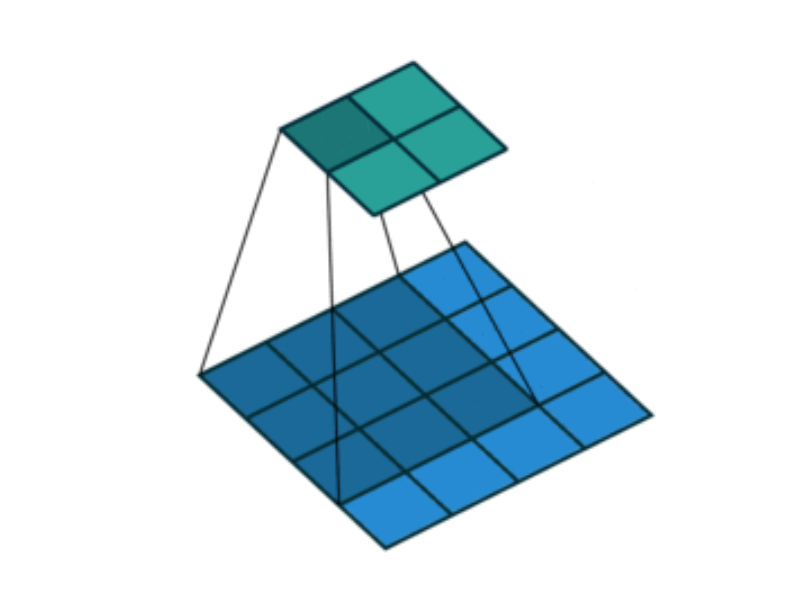
\includegraphics[width=0.4\textwidth]{images/convolution_operator}
       \caption{Aplicarea operatorului de convoluţie}
			\label{fig:convolution_operator}
       \source {\emph{A guide to convolution arithmetic for deep learning} \cite{dumoulin2016guide}}
    \end{center}
\end{wrapfigure}

Operatorul de convoluţie permite întelegerea datelor de intrare prin aplicarea unui kernel, ce extrage informaţia prin combinarea datelor asupra cărora este aplicat, fapt ilustrat în figura ~\ref{fig:convolution_operator}. Autoencoderele tradiţionale nu iau în considerare faptul că un semnal poate fi vazut ca o sumă de alte semnale. Operatorul de convoluţie a fost introdus în acestea tocmai pentru a exploata această posibilitate.  Autoencoderele convoluţionale reprezintă cea mai bună unealtă pentru învăţarea nesupravegheată a filtrelor convoluţionale. Spre deosebire de cazurile în care filtrele convoluţionale sunt construite manual pentru a extrage cât mai bine anumite trasături specifice din imagine, autoencoderele convoluţionale învaţă(construiesc) în mod automat filtrele în perioada de învăţare, având ca scop minimizarea erorii de reconstrucţie. Acestea reprezintă metoda perfectă pentru o obţine o reprezentare compactă a unor date abstracte si multi dimensionale, cum sunt imaginile digitale.\cite{goodfellow2016}
\par Obţinerea reprezentării latente a fiecărui obiect se realizează trecând imaginea, respectiv gradientul său prin encoderul autoencoderului corespunzător si păstrarea rezultatului.
\subsection{Clusterizare K-means}
\quad Odată obţinut vectorul de caracteristici pentru toate obiectele din setul de date, urmează stabilirea claselor de normalitate. Acest lucru se realizează prin aplicarea algoritmului k-means de clustering. Pentru implementare a fost folosit algoritmul \emph{LLoyd} implementat în biblioteca python \emph{sklearn}. Aplicând acest algoritm peste vectorii de caracteristici obţinuţi, rezultă k categorii de normalitate cu vectorii de caracteristici aferenţi. 
\par K-means este un tip de clusterizare ce are ca scop împărţirea a n probe în k grupe. Pentru ca grupele create să reprezinte clase de obiecte cât mai apropiate, algoritmul are ca scop minimizarea pătratului distanţei Euclidiene dintre probe. Algoritmul \emph{LLoyd} rezolvă această problema prin execuţia unei iniţializări (alegerea aleatorie a k centre) şi repetarea a doi paşi principali, până când problema converge la un minim local. Paşii executaţi sunt : 
\begin{itemize}
\item Atribuie fiecare element unei grupe. Elementul este atribuit grupei faţă de care criteriul de selecţie(pătratul distanţei Euclidiene faţă de centrul grupei) este minim.
\item Recalculează noi centre pentru fiecare grupa, pe baza noilor elemente. Centrele sunt calculate făcând media elementelor din fiecare grupă. 
\end{itemize}
\subsection{Clasificare multi-class folosind SVM}
\quad Folosind categoriile de normalitate obţinute la pasul anterior, putem spune că faţă de o anumită categorie \emph{i}, celelalte k-1 categorii reprezintă categorii \emph{artificial} anormale. Le numim \emph{artifical} anormale deoarece în mod obiectiv ele sunt acţiuni normale pentru sistemul de dectare a anomaliilor, dar pentru antrenarea unor clasificatori conform schemei one-vs-rest acestea sunt tratate drept anormale. Astfel, putem antrena un clasificator binar g(i) în aşa fel încat să separăm elementele din categoria i de cele din categoriile \{1,2...k\}/i 
generând funcţia : \[f_{i}(x) = \sum_{j  = 1}^{n} w_{j} * x_{j} + b\], unde x \(\in{R}^n\) reprezintă vectorul de caracteristici, w este vectorul de parametri a funcţiei, iar b reprezintă bias-ul funcţiei. \cite{ionescu2019object}.
\par Astfel, generăm k astfel de funcţii corespunzătoare celor k clasificatori ce vor fi folosiţi pentru a stabili daca un eveniment este anormal. Conform schemei one-vs-rest, un eveniment este anormal daca este clasificat drept anormal de către toţi cei k clasificatori.
\par Funcţia \(f_{i}\) reprezintă un SVM (maşină cu vectori suport) ce are ca scop clasificarea unor probe în diferite clase. În timpul perioadei de antrenare un SVM construieşte un hiperplan ce separă cât mai precis datele de antrenare în 2 clase conform etichetelor acestora, maximizând distanţa minimă faţă de planul de decizie. Astfel, scopul unei maşini cu vectori suport este găsirea unui \(\vec{w} \) minim(norma acestuia sa fie minimă)  astfel încât: \( y_{i}(\vec{w} \cdot \vec{x_{i}} - b) \ge 1, \quad \)pentru toţi \( 1 \le i \le n.\), unde \(y_{i} \) reprezintă eticheta probei \(x_{i}\). Ce înseamnă ca toate probele etichetate cu 1 se află de o parte a planului de decizie, şi toate probele etichetate cu -1 se află de cealaltă parte. 

\section{Etapa de inferenţă}
\quad În cadrul etapei de inferenţă, sistemul foloseşte detectorul de obiecte, autoencoderele pre-antrenate şi cei k clasificatori binari pentru a stabili dacă un anumit eveniment este sau nu anormal. Astfel, parcursul sistemului este următorul :
\begin{itemize}
\item Extragerea cadrelor necesare din video
\item Extragerea obiectelor din imagini
\item Obţinerea reprezentării latente
\item Clasificarea evenimentelor
\end{itemize}
\par
Pentru analiza unui eveniment care apare la un indice dat \emph{t} sunt necesare 3 cadre. Mai precis cadrele de la indicii \emph{t-3}, \emph{t+3} şi \emph{t}.
Din cadrul t se va extrage vectorul de caracteristici specific aparenţei vizuale, iar din celelalte 2 cadre se vor extrage vectorii de caracterisitici specifici mişcării obiectului, prin analiza gradienţilor. Prin concatenarea acestor 3 vectori, se obţine vectorul final de caracteristici ce va fi folosit drept input pentru clasificatorii finali.
\par
Pentru extragerea obiectelor din cadrele analizate, se va folosi acelaşi detector de obiecte ca în etapa de antrenare.  Acesta va fi rulat pe cadrul principal t, urmând apoi sa se folosească coordonatele obiectelor de la cadrul t, si pentru cadrele t+3 si t-3 deoarece din cauza diferenţei mici de indici, obiectele nu se pot mişca indeajuns incât sa fie necesară rularea pe toate cele 3 cadre.
\par
Odată obţinute obiectele din cadrul analizat, dupa obţinerea gradienţilor din cadrele t-3 si t+3, se poate obţine reprezentarea latentă a acestor informaţii.
Reprezentarea latentă a imaginii obiectului constă în rezultatul generat de encoderul autoencoderului pentru imagini iar reprezentarea latentă a gradienţilor constă în rezultatul generat de encoderul autoencoderului pentru gradienţi.
\par
Odată obtinuţi vectorii de caracteristici pentru reprezentarea vizuală şi pentru reprezentarea mişcării obiectului, prin concatenarea lor se obţine vectorul final, ce poate fi folosit drept input pentru clasificarea finală. Conform schemei \emph{one-vs-rest} acest vector este clasificat de toţi cei k clasificatori, iar rezultatul final este scorul maxim cu semn schimbat obţinut în urma clasificării.
\section{Etapa de lansare în cloud}
Pentru a face sistemul public, acesta este lansat drept un API ce rulează etapa de inferenţă pe un server web plasat in cloud. Pentru dezvoltarea serverului am ales să folosesc framework-ul \emph{Flask}. Flask este un micro-framework de python folosit pentru dezvoltarea soluţiilor web. Motivele pentru care acest framework a fost ales sunt : 
\begin{itemize}
\item Acesta adaugă un număr de dependeţe suplimentare foarte mic aplicaţiei, lucru esenţial atunci cand aplicaţia se doreşte a fi plasată în cloud, din cauza limitărilor de memorie. 
\item Oferă un suport foarte bun pentru planificarea rutelor de intrare în aplicaţie, lucru foarte important atunci când se doreşte dezvoltarea unui API.
\item Este unul dintre framework-urile suportate de Amazon Elastic Beanstalk 
\end{itemize}
\par
Comparativ cu alte framework-uri, Flask este diferit deoarece nu impune linii clare dezvoltatorilor atunci când vine vorba de forma sau componentele aplicaţiei ce urmează a fi dezvoltată. Astfel, dezvoltatorul are control complet asupra aplicaţiei si îşi poate manifesta creativitatea sau ideile fara a fi restricţionat de framework.  Flask a fost creat tocmai cu ideea de a fi construit peste el. Deşi poate nu oferă aceeaşi viteză de dezvoltare comparativ cu celelalte frameworkuri, acesta oferă libertatea de alegere la fiecare pas. Are suport pentru toate tipurile de baze de date, fie ele relaţionale sau nerelaţionale,  nu are preferinţe când vine vorba de metode de autentificare sau de creare a rolurilor, totul este suportat şi totul este la latitudinea dezvoltatorului. 
\cite{flask2014}
\par
Pentru a lansa serverul in cloud, am folosit serviciul Amazon Elastic Beanstalk. Acesta este un serviciu complex, ce însumează la rândul lui mai multe servicii cloud oferite de Amazon Web Services(AWS). Mai jos sunt prezentate câteva dintre avantajele şi dezavantajele acestui serviciu, fiind analizat în detaliu în capitolele ce urmează.  Elastic Beanstalk este un serviciu de tipul \emph{PaaS}  ce oferă servicii de deployment şi administrare complete.Pentru o mai bună detaliere, mai jos sunt definite toate serviciile cloud incluse de Elastic Beanstalk: 
\begin{itemize}
\item Amazon EC2 : este un serviciu web oferit de Amazon ce constă în oferirea unui mediu de execuţie sigur in cloud. Este echivalentul unei maşini fizice, doar că este accesată prin intermediul internetului. Acesta a fost creat pentru a uşura misiunea dezvoltatorilor de a migra serviciile proprii spre cloud computing.  Aceste instanţe sunt extrem de configurabile, punând la dispoziţia dezvoltatorului mai mult de 50 de tipuri de instanţe, plus diferite opţiuni de optimizare a unor părţi specifice, cum ar fi memoria sau placa video. \cite{2020EC2}
\item Amazon S3 : este un serviciu ce oferă medii de stocare în cloud. Stocarea este de tipul cheie-obiect, unde cheia identifică unic la nivel global un fişier. Acesta oferă o securitate sporită a datelor, şi o disponibilitate de 99.9999999\% deoarece datele sunt distribuite în sisteme diferite aflate în zone diferite.
\cite{2020S3}
\item Auto Scaling Group : acest serviciu oferă un mod automat de lansare a instanţelor EC2 astfel încât traficul să nu depăşească niciodata puterea de execuţie a unui aplicaţii. Scopul acestui serviciu este de a oferi capacitatea de a scala pentru a menţine o performanţă optimă, menţinând costul în tot acest timp la valoarea minimă.
\cite{2020autoscaling}
\item Elastic Load Balancing: este un serviciu care împarte traficul administrat de aplicaţie către instanţele lansate astfel încât acestea să fie utilizate intr-un. mod optim. Astfel, poate suporta încarcătura variabilă a aplicaţiei şi o poate distribui în aşa fel încat, în funcţie de modul ales(\emph {accesibilitate crescută}, \emph(scalare automată), \emph{securitate ridicată}) aplicaţia să nu scadă sub performanţele dorite.
\cite{2020elb}
\end{itemize}
\par 
\begin{figure}
\begin{center}
        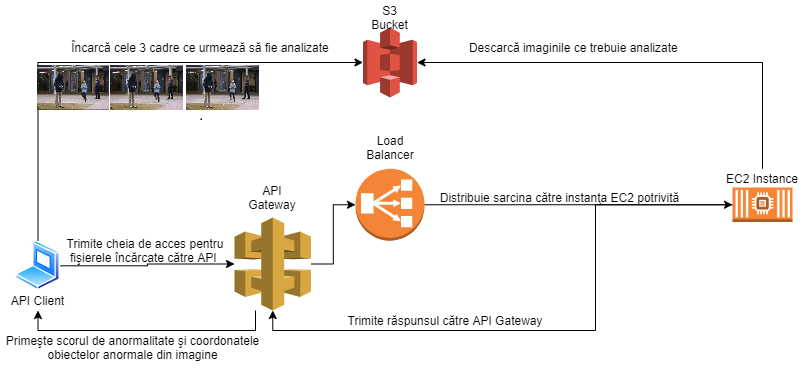
\includegraphics[width=1\textwidth]{images/client_drawing}
			 \caption{Arhitectura abstractizată a API-ului}
			 \label{fig:client_design}
\end{center}
\end{figure}

Dezvoltatorul se ocupă doar de aplicaţia/serverul propriu zis, crează pachetul de deployment, iar Elastic Beanstalk crează instanţele EC2 necesare, administrează şi rutează traficul către instanţe folosind un Load Balancer, iar atunci cand aplicaţia este suprasolicitată, lansează în mod automat noi servere folosindu-se de avantajele unui Auto Scaling Group.
\par Aşa cum se poate observa în figura ~\ref{fig:client_design}, API-ul este creat în aşa fel încât evaluarea se face pentru fiecare cadru în parte. Dezvoltatorul ce implementează clientul pentru API are doar responsabilitatea urcării cadrelor necesare într-un spaţiu S3 prestabilit. Preprocesarea, extragerea obiectelor din imagine, şi rularea detecţiei de anomalii sunt toate executate in cloud. Astfel, efortul computaţional asupra clientului este minim. La momentul accesării API-ului, serverul trebuie să primeasca ca parametru în apelul HTTP cheia de acces pentru cadrele urcate de catre client. Folosind această informaţie, pe server se descarcă aceste cadre şi sunt analizate pentru a detecta anomaliile din cadrul central. Ca şi rezultat, clientul primeşte scorul de anormalitate al cadrului împreună cu toate poziţiile obiectelor anormale din cadru, date ce pot fi folosite pentru notificări ulterioare sau diferite aplicaţii pe partea de client. Un avantaj important al unui HTTP API este abilitatea de a fi accesat prin internet, interfaţa API-ului fiind accesibilă pentru toţi utilizatorii fară să necesite instrucţiuni speciale, precum \emph{SOAP} ce este bazat pe \emph{XML}.

\section {Tehnologii folosite în dezvoltarea interfeţei}
\quad Pentru a putea vizualiza capacităţile sistemului de detecţie a anomaliilor, am dezvoltat un program ce simulează cele 2 moduri în care poate fi acesta sistem folosit : prin rulare locală, sau prin execuţie în cloud.
\par Pentru a creea interfaţa grafică, am ales să folosesc framework-ul \emph{Electron}. Electron este un framework creat pentru a facilita dezvoltarea de aplicaţii desktop cross-platform, folosind tehnologii web. Acesta este bazat pe \emph{Node.js} şi \emph{Chromium} şi pune la dispoziţia dezvoltatorului folosirea tehnologiilor web precum: 
\begin{itemize}
\item{HTML}
\item{CSS}
\item{JavaScript}
\end{itemize}
\par
Datorită posibilităţii de a folosi tehnologii web pentru a dezvolta interfaţa unei aplicaţii desktop, se pot crea interfeţe atractive, stilizate şi aranjate astfel încât experienţa utilizării programului să fie cât mai bună. 
\begin{figure}[h]
\begin{center}
        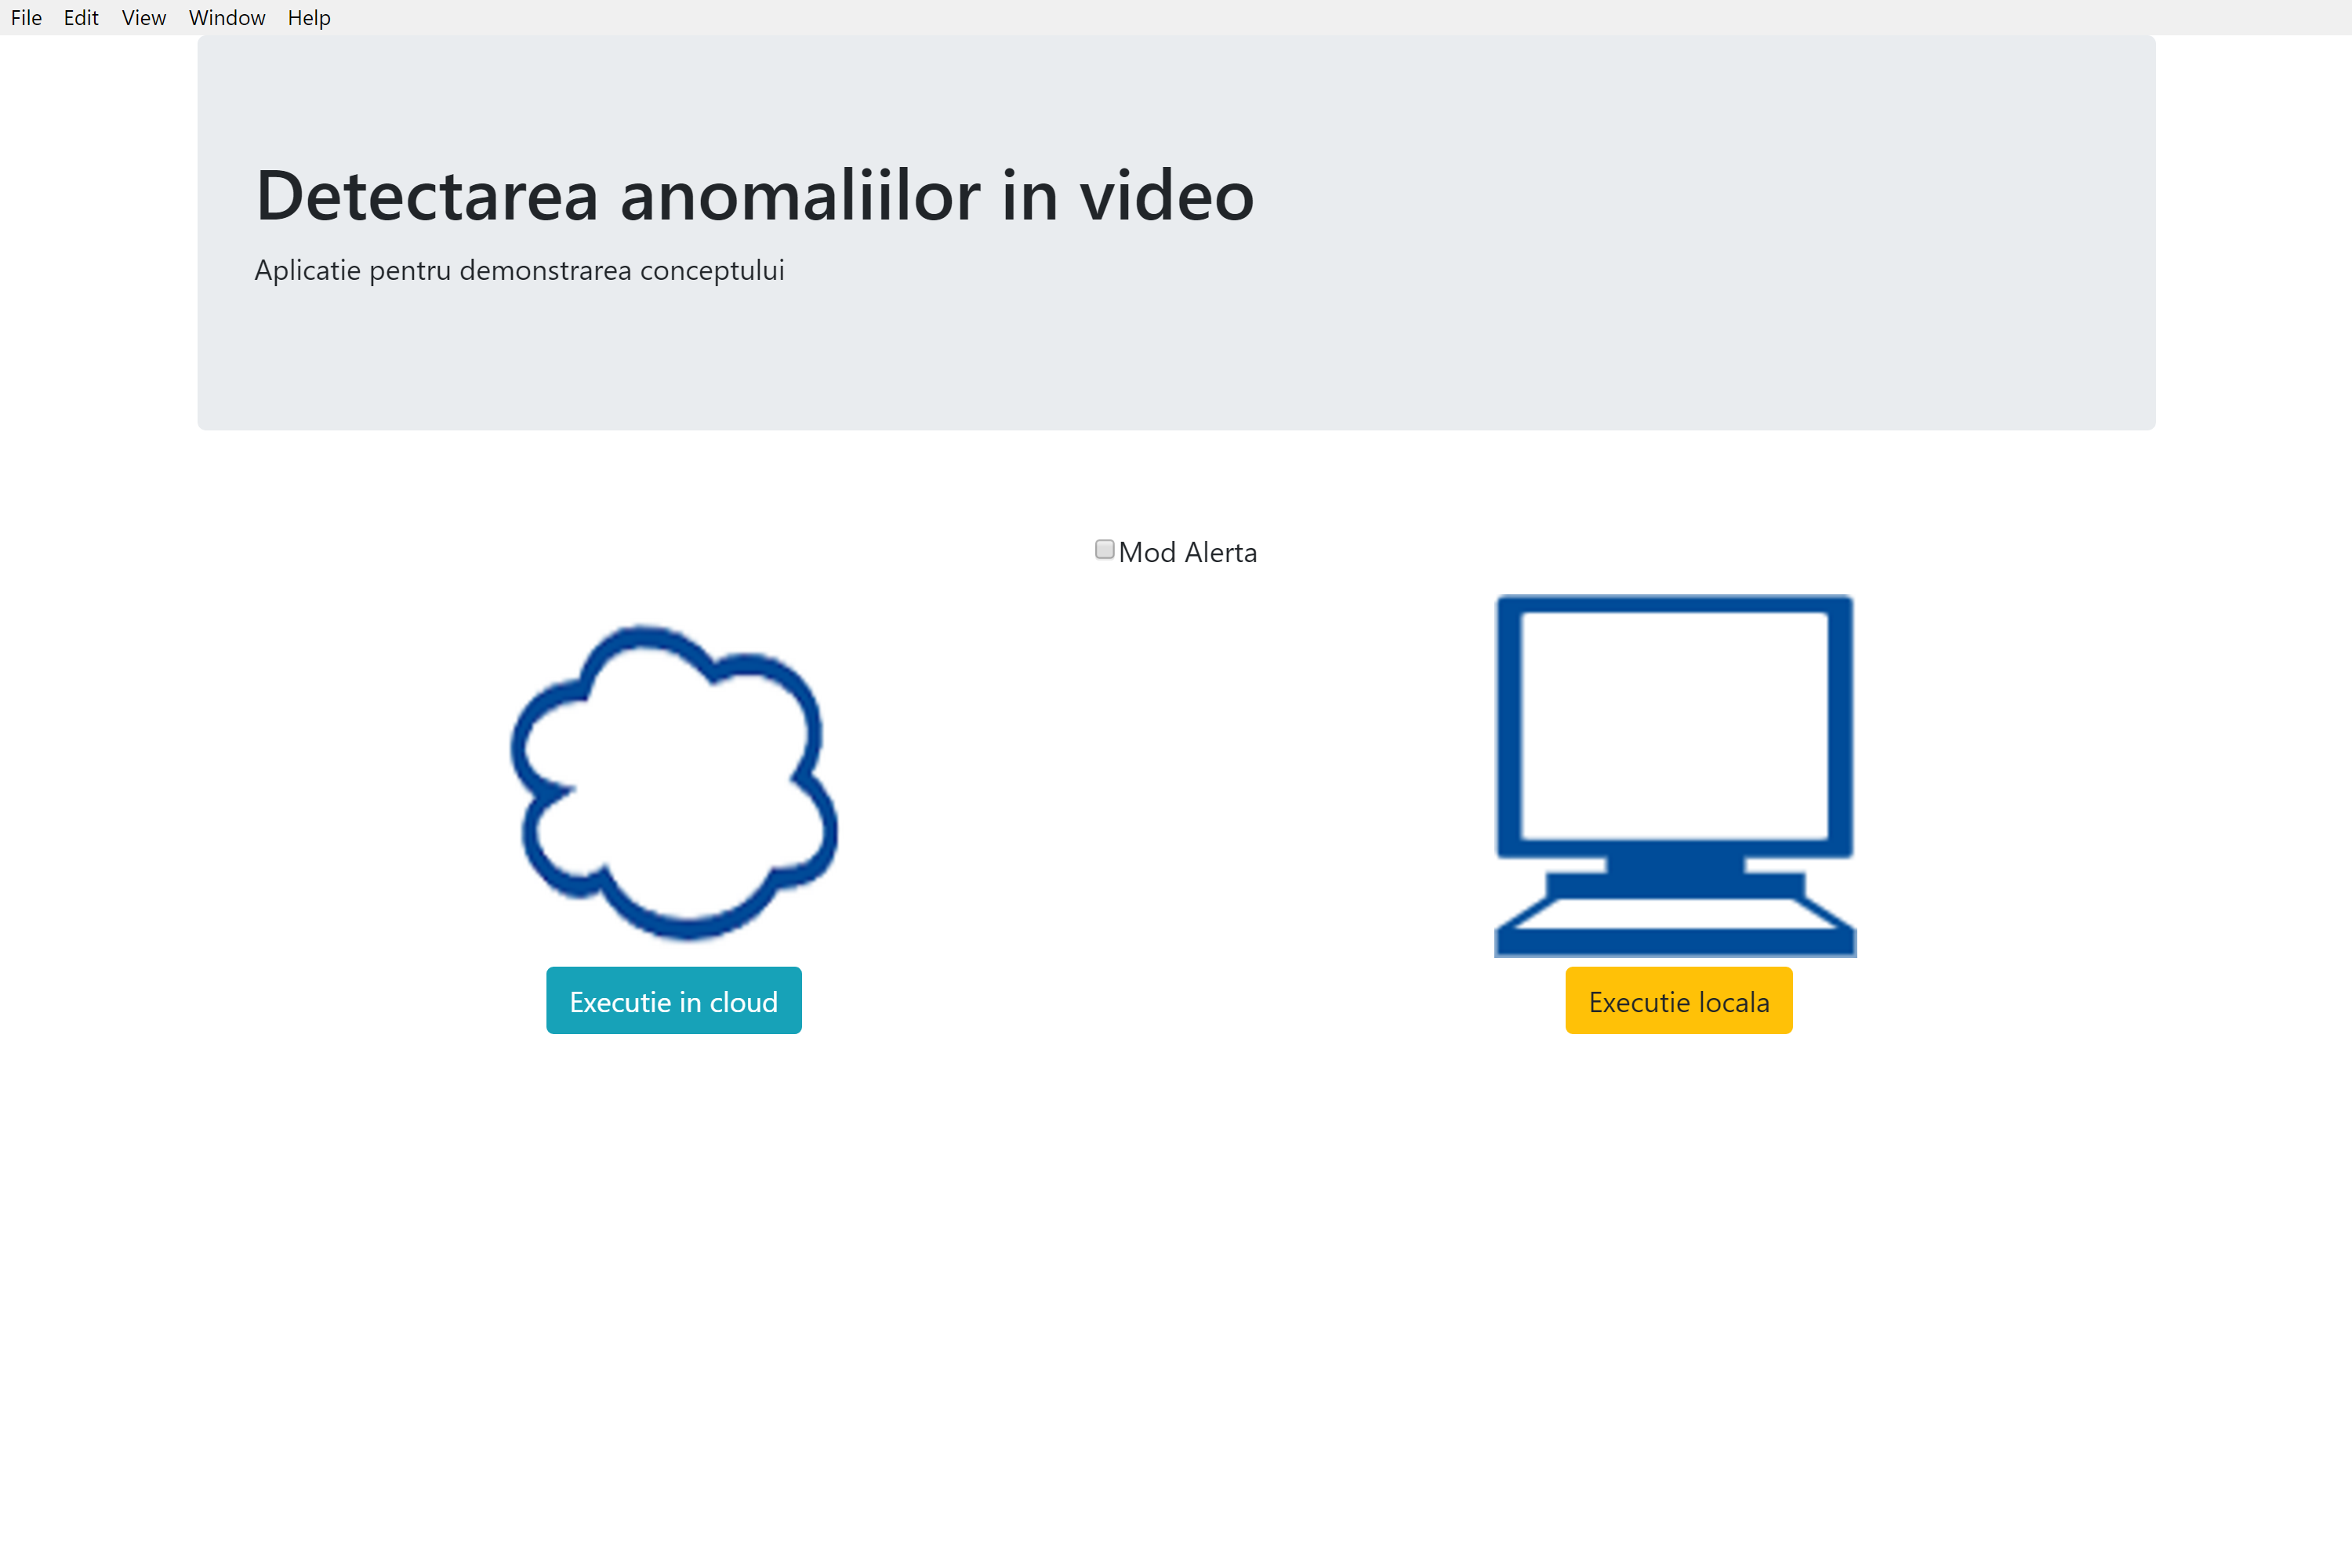
\includegraphics[width = 1\textwidth]{images/interfata}
			 \caption{Pagina de start a aplicaţiei}
			 \label{fig:interfata}
\end{center}
\end{figure}
\par Programul creat simulează un client ce foloseşte sistemul de detecţie a anomaliilor şi anume : rulează detecţia de anomalii (local sau în cloud, în funcţie de metoda selectată) folosind o cameră video ataşată sistemului de pe care este rulat. Modul în care sunt evidenţiate evenimentele anormale este deasemenea configurabil :
\begin{itemize}
\item Modul standard : Încadrarea în cadrane verzi a obiectelor ce sunt detectate de către sistem ca având un comportament anormal. 
\item Modul alertă : Programul extrage obiectul din imagine atunci cand acesta este detectat ca fiind anormal, şi creează o alertă conţinând doar această imagine pe care o afişează pe ecran. Acest mod de alertă simulează scenariul în care este necesară atragerea atenţiei în mod suplimentar a operatorului în momentul apariţiei unei anomalii.  
\end{itemize}

\chapter{Sistemul de detecţie a anomaliilor}
\quad În acest capitol va fi analizat în detaliu sistemul de detecţie a anomaliilor în video, atât din punct de vedere al arhitecturii alese cât şi din punct de vedere al implementării.
\section{Detecţia obiectelor}
\par În ceea ce priveşte detecţia de obiecte, aceasta este comună tuturor etapelor sistemului. Aşa cum se poate observa şi in secţiunea de analiză a performanţelor sistemului,detecţia obiectelor din imagine joacă un rol esenţial în viteza finală de analiză. 
\par Prima opţiune a fost un detector de obiecte pre-antrenat pe setul de date COCO ce foloseşte o arhitectură \textbf{SSD-Mobilenet}, din biblioteca \emph {gluoncv model-zoo}. Acesta are ca prim avantaj viteza de analiză pe GPU a unei imagini, dar şi precizia bună a detecţiilor. Fiind asemănător cu cel folosit de \emph{Ionescu et al.}, acesta foloseşte o arhitectură ce poate fi exploatată la potenţialul ei maxim doar pe o maşina ce posedă un GPU puternic, având o viteza insuficientă pe sisteme bazate doar pe CPU. 
\par Deoarece sistemul actual are ca scop final rularea pe o platforma ce necesită resurse minime, atât in cazul rulării offline cât şi online, am ales folosirea unui model cu o arhitectură optimizată pentru rularea pe CPU. Mai precis, un model cu o arhitectură \textbf{YOLOv3-tiny} preluat din biblioteca \emph{libcv}.
Această schimbare a adus o imbunatăţire de \textbf{10x} în ceea ce priveşte timpul de detecţie a obiectelor per cadru, de la o medie de  1200 de ms la 120 ms.
\par Detectorul YOLO este un tip de detector cu o singură etapă, ceea ce semnifică ca nu mai este executată etapa de propunere a regiunilor întalnite în detectoarele cu 2 etape, precum \emph{R-CNN} sau \emph{Fast R-CNN}. Astfel, imaginea este împarţită în \( S \times S \) pătrate. Fiecare pătrat este responsabil să detecteze obiectul aflat în interiorul acestuia.Fiecare pătrat are atribuit un scor ce arată probabilitatea ca un obiect să se afle în acesta, şi încă un scor, ce reprezintă intersecţia supra reuniune dintre perimetrul prezis şi poziţia adevărată a obiectulului din imagine.   Pentru fiecare astfel de pătrat sunt propuse \emph{bounding box-uri} şi scorul de încredere aferent. Un astfel de detector are la bază nivele convoluţionale ce extrag caracteristici din imagine urmată de nivele conectate complet pentru clasificare. Desigur, YOLOv3-tiny a suferit numeroase modificări în scopul optimizării arhitecturii din punct de vedere al timpului de execuţie.\cite{jiao2019}
Odată cu viteza apare în schimb un dezavantaj în ceea ce priveşte detecţia de obiecte: datorită arhitecturii minimaliste, detectorul ales detecteză obiectele în integritatea lor doar dacă sunt relativ aproape de cameră şi nu sunt foarte mici. 
\par Implementarea detecţiei de obiecte a fost realizată la nivelul sistemului în cadrul clasei \emph{ObjectDetector} ce prezintă următoarele funcţionalităţi :
\begin{itemize}
\item La momentul instanţierii rulează detectorul de obiecte pre-antrenat pe imaginea primită ca parametru, obţinând astfel cadranele delimitatoare ale obiectelor din imagine împreuna cu scorurile şi clasele aferente. 
\item Oferă prin intermediul funcţiei \emph{get\_object\_detections} obiectele extrase din imagine pe baza marginilor delimitatoare obţinute în timpul instanţierii. Obiectele sunt redimensionate la \( 64 \times 64\) şi returnate sub forma unui vector de imagini.
\item Oferă prin intermediul funcţiei \emph{get\_detections\_and\_cropped\_sections} ce primeşte ca parametru şi imaginea de la indexul t-3 si imaginea de la indexul t + 3 relativ la indexul t  al imaginii folosite pentru instanţiere pachetul complet pentru trecerea prin sistemul de detecţie şi anume : Folosind marginile delimitatoare obţinute în timpul instanţierii, sunt extrase obiectele din toate cele 3 imagini, şi returnate sub forma a 3 vectori de imagini. Astfel un eveniment va fi format din cele 3 imagini aflate la un acelaşi index \emph{i} în cei 3 vectori. 

\end{itemize}
\section{Analiza antrenării sistemului}
\quad Din cauza complexităţii problemei de a identifica comportamentul anormal al obiectelor prezente în video, arhitectura sistemului presupune multiple etape de prelucare a datelor până la momentul clasificării finale. Astfel, etapa de antrenare este împărţită la rândul ei în 2 etape:
\begin{itemize}
\item Etapa de reducere a dimensionalităţii (antrenarea autoencoderelor)
\item Etapa de antrenare a clasificatorilor finali
\end{itemize}
\begin{figure}[h]
\begin{center}
        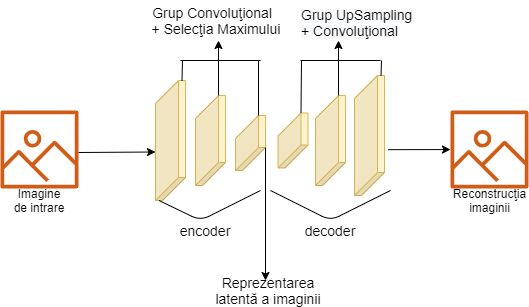
\includegraphics[width=1\textwidth]{images/arhitectura_autoencoder}
			 \caption{Prezentarea principiului de funcţionare a autoencoderelor şi arhitectura lor generală}
			 \label{fig:arhitectura_autoencoder}
\end{center}
\end{figure}
\par În etapa de reducere a dimensionalităţii sunt definite şi antrenate autoencoderele pe baza imaginilor si gradienţilor extraşi din setul de date. Motivul pentru care obiectele sunt procesate de către autoencodere este că datorită antrenării doar pe obiectele din videourile de antrenare, acestea vor învăţa să reprezinte mai bine evenimentele normale. Astfel, atunci cand prin aceste autoencodere vor trece evenimente anormale, ce nu sunt asemanătoare cu cele de antrenament, autoencoderele vor genera o eroare de reconstrucţie ce va uşura sarcina clasificatorilor finali.
\par Arhitectura aleasă pentru autoencodere este cea descrisă de \emph{Ionescu et al.}  \cite{ionescu2019object} şi constă intr-o arhitectură convoluţională rapidă, formată dintr-un encoder cu 3 blocuri convoluţional + max-pooling şi un decoder format din 3 blocuri upsampling + convoluţional. Fiecare autoencoder primeşte ca input date de dimensiune \(64 \times 64\) si creează după encoder un vector de caracteristici de dimensiune \(8 \times 8 \times 16\).  Structura detaliată a autoencoderelor este : 
\begin{itemize}
\item Stratul de intrare, de dimensiune \( 64 \times 64 \times 1\)
\item Bloc  Convoluţional + MaxPooling format din : Un strat convoluţional bazat pe 32 de filtre de dimensiune \(3 \times 3\) urmat de funcţia de activare \emph{Relu} şi un strat max-pooling bazat pe filtre \(2 \times 2\) cu \emph{stride} 2.
\item Bloc  Convoluţional + MaxPooling format din : Un strat convoluţional bazat pe 32 de filtre de dimensiune \(3 \times 3\) urmat de funcţia de activare \emph{Relu} şi un strat max-pooling bazat pe filtre \(2 \times 2\) cu \emph{stride} 2.
\item Bloc  Convoluţional + MaxPooling format din : Un strat convoluţional bazat pe 16 de filtre de dimensiune \(3 \times 3\) urmat de funcţia de activare \emph{Relu} şi un strat max-pooling bazat pe filtre \(2 \times 2\) cu \emph{stride} 2.
\item Bloc Convoluţional + UpSampling fprmat din : Un strat convoluţional bazat pe 16 de filtre de dimensiune \(3 \times 3\) urmat de funcţia de activare \emph{Relu} şi un strat UpSampling bazat pe filtre \(2 \times 2\).
\item Bloc Convoluţional + UpSampling fprmat din : Un strat convoluţional bazat pe 32 de filtre de dimensiune \(3 \times 3\) urmat de funcţia de activare \emph{Relu} şi un strat UpSampling bazat pe filtre \(2 \times 2\).
\item Bloc Convoluţional + UpSampling fprmat din : Un strat convoluţional bazat pe 32 de filtre de dimensiune \(3 \times 3\) urmat de funcţia de activare \emph{Relu} şi un strat UpSampling bazat pe filtre \(2 \times 2\).
\item Un ultim strat Convoluţional ce are ca rol reducerea dimensiunii de ieşire de la \(64 \times 64 \times 32\) la \(64 \times 64 \times 1\)\cite{ionescu2019object} .  Aceste este bazat pe 1 filtru de dimensiune \(3 \times 3 \) urmat de funcţia de activare \emph{Sigmoid}
\end{itemize}
Primele 4 straturi reprezintă encoder-ul, în timp ce ultimele 4 straturi reprezintă decoderul. 
\par În cadrul sistemului, clasa \emph{AutoEncoderModel} implementează funcţionalităţile necesare şi anume : 
\begin{itemize}
\item La momentul instanţierii defineşte arhitectura autoencoderului. 
\item Prin intermediul metodei \emph{\_\_train\_autoencoder} antrenează autoencoderul pe baza unui vector de imagini primit ca parametru. Inainte de a incepe antrenarea propriu zisă se verifică dacă există deja un model pre-antrenat în sistemul de fişiere. Daca nu există, se realizează antrenarea completă, urmată de salvarea modelului în sistemul de fişiere.
\item Prin intermediul metodei \emph{get\_encoded\_state} ce primeşte ca parametru o imagine, returnează reprezentarea latentă a acelei imagini. 
\end{itemize}
Implementarea clasei \textbf{AutoEncoderModel} este : 
\begin{footnotesize}
\begin{lstlisting}
class AutoEncoderModel:
    """
    ----------
    autoencoder = Modelul pentru autoencoderul complet, 
    contine atat encoderul cat si decoderul
    encoder = doar encoderul, extras din autoencoder,avand aceleasi greutati.
    """
    def __init__(self, input_images, checkpoints_name):
        self.checkpoints_name = checkpoints_name
       #fisierul in care vor fi salvate modelele dupa antrenare
        self.checkpoint_dir = '/home/some_directory_%s' % self.checkpoints_name
        self.num_epochs = 100
        self.batch_size = 64
        self.autoencoder, self.encoder = self.__generate_autoencoder()
        self.__train_autoencoder(input_images)

    def __generate_autoencoder(self):
        input_img = Input(shape=(64, 64, 1))
        x = Conv2D(32, (3, 3), activation='relu', padding='same')(input_img)
        x = MaxPooling2D((2, 2), strides=2, padding='same')(x)
        x = Conv2D(32, (3, 3), activation='relu', padding='same')(x)
        x = MaxPooling2D((2, 2), strides=2, padding='same')(x)
        x = Conv2D(16, (3, 3), activation='relu', padding='same')(x)
        encoded = MaxPooling2D((2, 2), strides=2, padding='same')(x)
        x = Conv2D(16, (3, 3), activation='relu', padding='same')(encoded)
        x = UpSampling2D((2, 2))(x)
        x = Conv2D(32, (3, 3), activation='relu', padding='same')(x)
        x = UpSampling2D((2, 2))(x)
        x = Conv2D(32, (3, 3), activation='relu', padding='same')(x)
        x = UpSampling2D((2, 2))(x)
        decoded = Conv2D(1, (3, 3), activation='sigmoid', padding='same')(x)
        autoencoder = Model(input_img, decoded)
        encoder = Model(input_img, encoded)
        # compileaza modelele folosind optimizatorul Adam si 
        # diferenta medie patratica drept functie loss
        optimizer = Adam(lr=10 ** -3)
        encoder.compile(optimizer=optimizer, loss='mse')
        autoencoder.compile(optimizer=optimizer, loss='mse')
        print(autoencoder.summary())
        return autoencoder, encoder

    def __train_autoencoder(self, input_images):
        """
        Parametri
        ----------
        input_images = np.array ce contine imagini de dimensiune 64x64x1
        ce vor fi folosite pentru a antrena autoencoderul
        """
        if not os.path.exists(self.checkpoint_dir):
            os.makedirs(self.checkpoint_dir)
            checkpoint_callback = 
		ModelCheckpoint(filepath=self.checkpoint_dir + '/weights.hdf5', 
			verbose=1,
			save_best_only=True)
            early_stopping_monitor = EarlyStopping(patience=2)
            data_train, data_test, gt_train, gt_test = 
		train_test_split(input_images, input_images, test_size=0.20,
			random_state=42)
            self.autoencoder.fit(data_train, data_train,
                          epochs=self.num_epochs,
                          batch_size=self.batch_size,
                          validation_data=(data_test, data_test),
                          callbacks=[checkpoint_callback, early_stopping_monitor])
        else:
            self.autoencoder.load_weights(self.checkpoint_dir + '/weights.hdf5')

    def get_encoded_state(self, image):
        """
        Parametri
        ----------
        images - np.array ce contine imaginea ce trebuie codificata 
        Rezultat
        -------
        np.array ce contine imaginea codificata de catre encoder
        """
        input = np.expand_dims(image,axis = 0)
        encodings = self.encoder.predict(input)
        return encodings[0]
\end{lstlisting} \cite{2020autoencoders}
\end{footnotesize}
\begin{figure}[h]
\begin{center}
        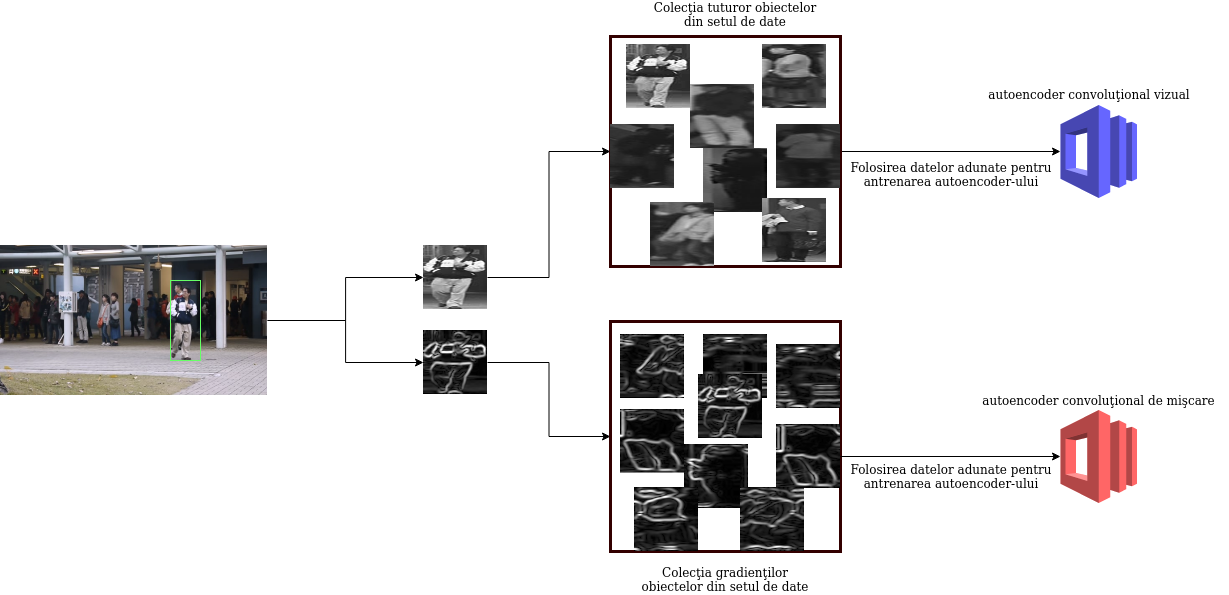
\includegraphics[width=1\textwidth]{images/training_stage1_architecture}
			 \caption{Arhitectura primei etape de antrenare}
			 \label{fig:stage1_architecture}
\end{center}
\end{figure}
\par
Implementarea arhitecturii prezentate în figura ~\ref{fig:stage1_architecture} constă în următorii paşi:
\begin {itemize}
\item Pentru toate videourile de antrenare se execută detecţia de obiecte pentru fiecare cadru, extrăgând astfel toate obiectele din video.Fiecare cadru este transformat în alb-negru pentru a fi prelucrat în etapele următoare. Pentru fiecare obiect extras, imaginea acestuia este redimensionată pentru a respecta dimensiunea de intrare a autoencodere-lor la \( 64 \times 64 \) iar apoi este calculat gradientul, ce reflectă mişcarea obiectului. Gradientul este calculat după formula: \[\sqrt{G_{x}^2 + G_{y}^2}\] Unde \(G_{x}\), \(G_{y}\) sunt imagini ce în fiecare punct conţin derivata orizontală respectiv verticală a imaginii iniţiale, obţinută prin aplicarea unui kernel Sobel de \(3 \times 3 \).
\par Dimensiunea kernelului folosit pentru calcularea gradienţilor este foarte importantă pentru extragerea precisă a detaliilor, deoarece, asa cum se poate observa in figura ~\ref{fig:gradient_kernel}, cu cât kernelul este mai mare, cu atât trasaturile extrase sunt mai generale.
\item Imaginile şi gradienţii astfel obţinuţi sunt adaugaţi într-o colecţie generală pentru tot setul de date. Cele 2 colecţii astfel create vor servi drept input pentru antrenarea autoencoderelor.
\item Folosind cele 2 colecţii (de imagini, respectiv de gradienţi) este antrenat câte un autoencoder pentru fiecare colecţie. Înainte de a fi folosite pentru antrenarea autoencoderelor, atât imaginile, cât şi gradienţii, sunt normalizate în intervalul [0,1] .Antrenarea se realizează folosind optimizatorul Adam \cite{adam2017} şi funcţia loss ce constă în diferenţa medie a pătratelor, dată de formula : 
\(L(I,O) = \frac{1} {h*w} \sum_{1}^{h} \sum_{1}^{w} (I_{ij} - O_{ij})^2 \)   \cite{ionescu2019object} unde I şi O reprezintă imaginea de input respectiv de output şi h,w sunt dimensiunile imaginilor. Aceasta este executată timp de 100 de epoci cu o rată de învăţare de \(10^{-3}\), dar având şi o regula de oprire rapidă, ce inseamnă că dacă timp de 2 epoci funcţia loss nu se imbunătaţeşte, antrenarea este finalizată.
\end{itemize}

\begin{wrapfigure}{r}{0.45\textwidth}
	  \begin{center}
        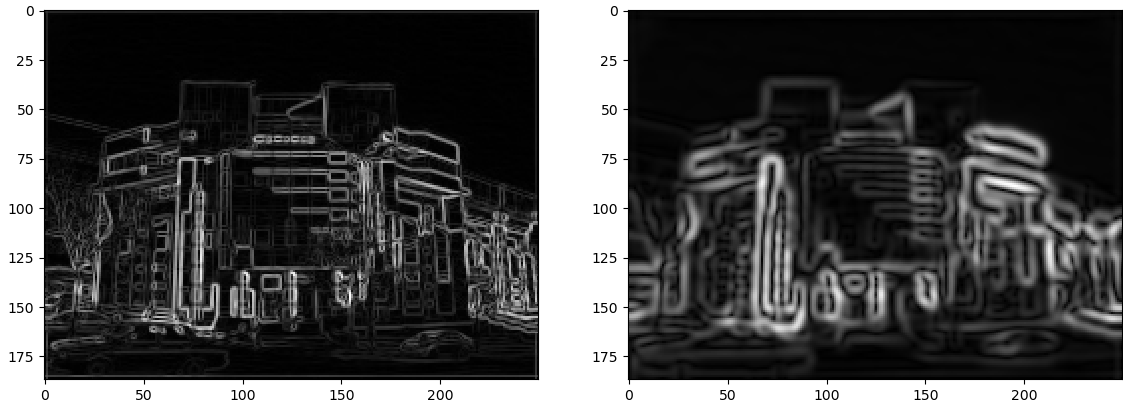
\includegraphics[width=0.4\textwidth]{images/gradients}
        \caption{Gradienţi obţinuţi în urma aplicării unui kernel \(3 \times 3 \), respectiv unul de dimensiune   \(21 \times 21 \)}
			\label{fig:gradient_kernel}
    \end{center}
\end{wrapfigure}
\par
În etapa de antrenare a clasificatorilor finali, se folosesc autoencoderele antrenate în etapa precedentă pentru a obţine vectorii de caracteristici specifici fiecărui eveniment prezent în setul de date. Ca şi prim pas, se detectează toate obiectele prezente în fiecare cadru din video-urile  de antrenare, iar pentru fiecare obiect, se folosesc coordonatele acestuia pentru a decupa acelaşi obiect din cadrul \emph{t-3} şi \emph{t+3}, respectiv la indexul \emph{t} curent. Se calculează gradienţii pentru imaginile decupate, astfel este reprezentată mişcarea obiectului faţă de cadrul curent, iar apoi se obţin vectorii caracteristici ai fiecarui gradient prin trecerea acestora prin autoencoderul corespunzător antrenat în etapa precendentă. Odată obţinuţi cei 3 vectori caracteristici specifici evenimentului, aşa cum este ilustrat şi în figura ~\ref{fig:stage2_architecture}, concatenarea acestora este stocată într-o colecţie globală ce reţine datele pentru tot setul de date.
Obţinerea vectorului de caracterisitici pentru un anumit eveniment este realizată în cadrul funcţiei :
\\
\begin{footnotesize}
\begin{lstlisting}
def __get_feature_vectors_and_bboxes(self, frame, frame_d3, frame_p3):
      """
      :param frame: np.array - Cadrul ce trebuie analizat
      :param frame_d3 : np.array - Cadrul de la indexul t-3 comparativ 
      cu indexul t al cadrul ce trebuie analizat. d3 vine de la delta3
      :param frame_p3 : np.array  - Cadrul de la indexul t+3 comparativ 
      cu indexul t al cadrul ce trebuie analizat. p3 vine de la plus3
      """
      object_detector = ObjectDetector(frame)
      bounding_boxes = object_detector.bounding_boxes
      cropped_detections, cropped_d3, cropped_p3 = 
	object_detector.get_detections_and_cropped_sections(frame_d3,frame_p3)
      gradient_calculator = GradientCalculator()
      gradients_d3 = 
	self.__prepare_data_for_CNN(gradient_calculator
			.calculate_gradient_bulk(cropped_d3))
      gradients_p3 = 
	self.__prepare_data_for_CNN(gradient_calculator
			.calculate_gradient_bulk(cropped_p3))
      cropped_detections = self.__prepare_data_for_CNN(cropped_detections)
      list_of_feature_vectors = []
      for i in range(cropped_detections.shape[0]):
          apperance_features = 
          self.trainer_stage2.autoencoder_images
			.get_encoded_state(np.resize(cropped_detections[i]
						, (64, 64, 1)))
          motion_features_d3 = self.trainer_stage2.autoencoder_gradients
			.get_encoded_state(np.resize(gradients_d3[i]
						, (64, 64, 1)))
          motion_features_p3 = self.trainer_stage2.autoencoder_gradients
			.get_encoded_state(np.resize(gradients_p3[i]
						, (64, 64, 1)))
          feature_vector = 
		np.concatenate((motion_features_d3.flatten()
		,apperance_features.flatten()
		, motion_features_p3.flatten()))
          list_of_feature_vectors.append(feature_vector)
      return np.array(list_of_feature_vectors),bounding_boxes
\end{lstlisting}
\end{footnotesize}
\begin{figure}[h]
\begin{center}
        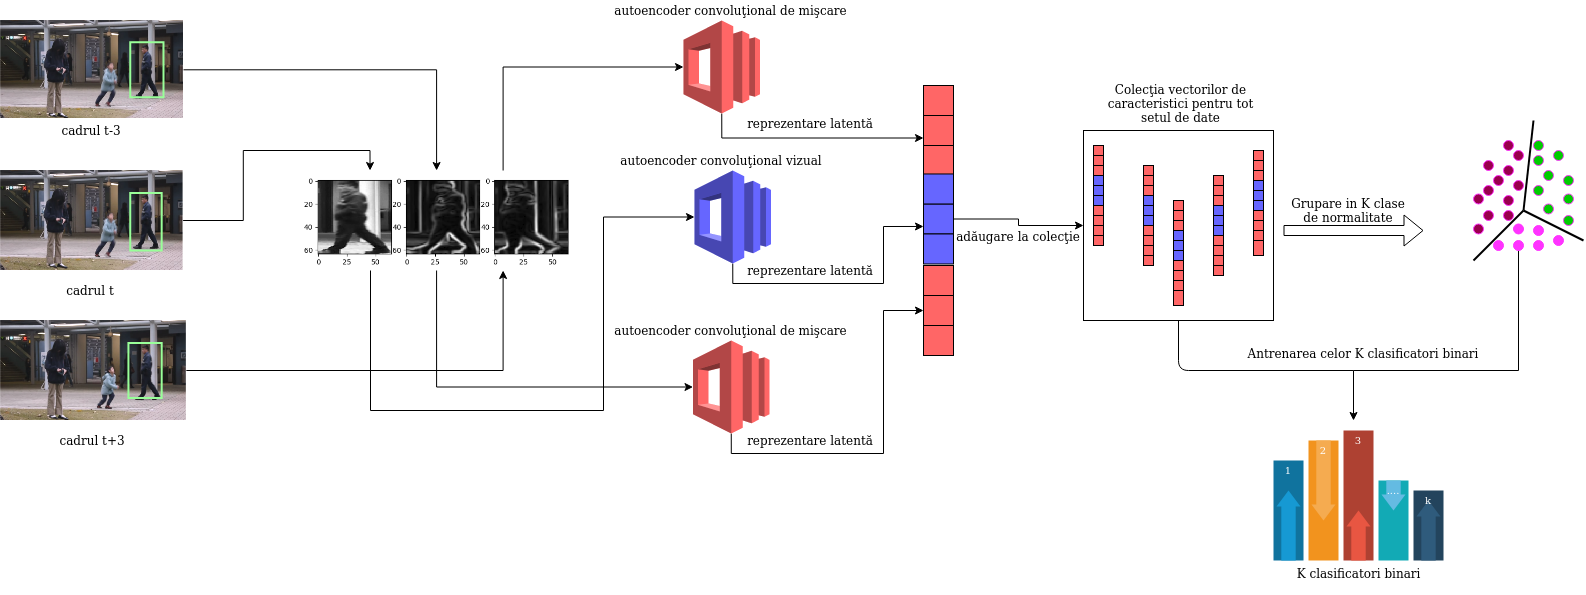
\includegraphics[width=1\textwidth,height=8cm]{images/training_stage2_architecture}
			 \caption{Arhitectura etapei finale de antrenare}
			 \label{fig:stage2_architecture}
\end{center}
\end{figure}
\par
Aplicând algoritmul de \emph{k-means clustering} se obţin k categorii de normalitate. Astfel, pentru fiecare eveniment din colecţia globală este cunoscută categoria \emph{i} din care face parte. Folosind aceste date, putem antrena cei k clasificatori binari. Pentru fiecare categorie, un clasificator binar este antrenat folosind evenimentele din categoria curent drept date de antrenare pozitive, iar celelalte k-1 categorii drept date de antrenare negative. În final, se obţin k clasificatori binari ce au rolul de a evalua daca un eveniment aparţine sau nu categoriei de normalitate \emph{i} unde \emph{i} este indicele clasificatorului 
\emph{\(g_{i}\)}. 
\par Ca şi implementare, antrenarea sistemului a fost dezvoltată având ca scop creearea unui flux de lucru automat şi configurabil. Astfel, pentru a reantrena sistemul folosind un alt set de date, este necesară doar schimbarea parametrului ce conţine calea către video-urile de antrenament.
\section{Analiza etapei de inferenţă}
În cadrul etapei de inferenţă este analizat un eveniment cu scopul de a determina dacă acesta este sau nu anormal. Analiza unui singur eveniment stă la baza tuturor modurilor de utilizare a sistemului, deoarece, având aceste date, putem obţine scoruri de normalitate pentru fiecare cadru, sau scoruri de normalitate la nivel de pixel sau chiar şi clasificări generale de normalitate a unui video în totalitate.

\begin{figure}[h]
\begin{center}
        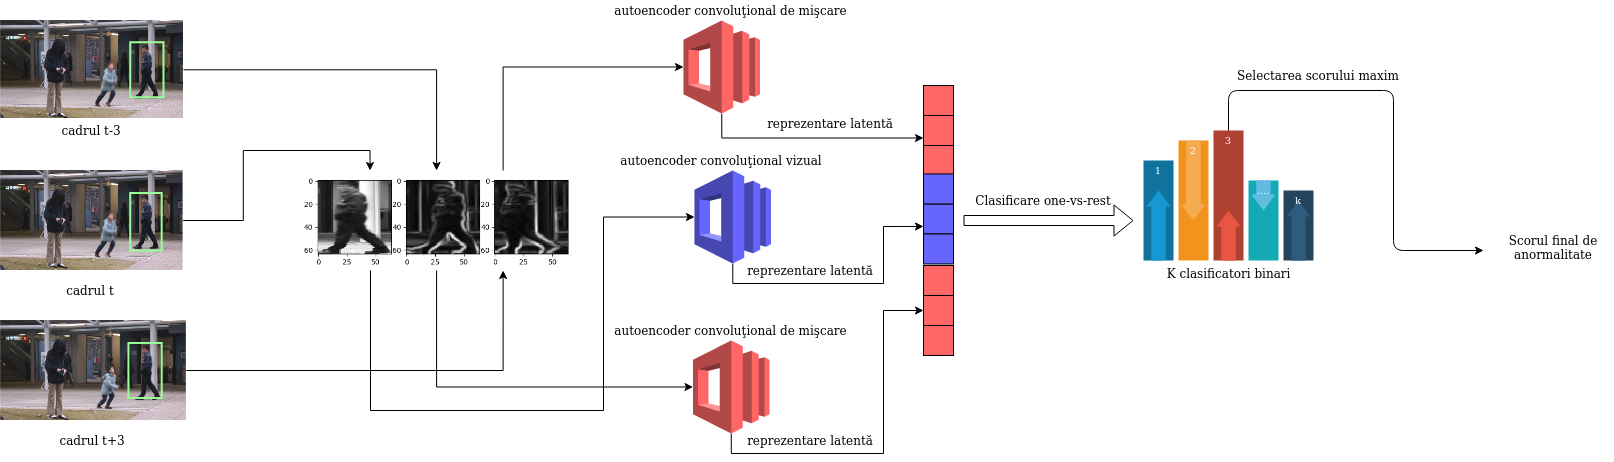
\includegraphics[width=1\textwidth,height=6cm]{images/inference_architecture}
			 \caption{Arhitectura etapei de inferenţă}
			 \label{fig:inference_architecture}
\end{center}
\end{figure}
Pentru a obţine scorul unui eveniment, un pas foarte important este obţinerea vectorului de caracteristici corespunzător. Acesta se obţine folosind autoencoderele antrenate în etapa precedentă, după pre-procesarea cadrelor corespunzătoare evenimentului.  Pre-procesarea este asemanătoare etapei de antrenare, şi anume, pentru fiecare obiect dintr-un cadrul \emph{t}, se selectează aceeaşi zonă din cadrele \emph{t-3} si \emph{t+3} cu scopul de a calcula gradienţii ce reflectă mişcarea obiectului relativ la cadrul t. Odată obţinute aceste 3 date (imaginea obiectului şi cei 2 gradienţi) aşa cum este descris şi in figura
~\ref{fig:inference_architecture}, acestea sunt trecute prin autoencodere şi sunt obţinute reprezentările latente, ce sunt concatenate pentru a se obţine vectorul final de caracteristici. Vectorul de caracteristici este apoi clasificat de toţi cei k clasificatori binari antrenaţi anterior, iar scorul final de anormalitate este dat de formula : \[score = -max(g_{i}(v)), i \in [1..k]\] unde v este vectorul de caracteristici, iar \(g_{i}\) este un clasificator binar.
Implementarea funcţiei ce generează scorul de anomalie a unui eveniment este : 
\begin{lstlisting}
 def get_inference_score(self,feature_vector):
        scores = self.model.decision_function([feature_vector])[0]
        return -max(scores)
\end{lstlisting}
\par
Filmarea propriu zisă şi selecţia cadrelor este realizată pe partea de client, în timp ce pre-procesarea cadrelor, detecţia obiectelor şi calcularea scorului pentru fiecare dintre aceste obiecte este executat pe server. Astfel, atât timp cât există o conexiune la reţea, clientul nu este limitat de puterea de calcul proprie, şi poate analiza mai multe videouri simultan. Totuşi clientul trebuie sa încarce cadrele ce vor fi analizate catre o destinaţie S3 a serverului. Pentru a nu încetini semnificativ procesul de analiză, trimitere cadrelor în reţea trebuie facută în paralel, folosind eventualele posibilităţi de multi-threading ale clientului.
\par
În ceea ce priveşte serverul pe care rulează analiza propriu zisă, acesta este un HTTP API, ce expune pentru public capacitatea de a rula inferenţa. În stadiul curent, API-ul este configurat cu un singur endpoint, de tip POST  : \say{upload/frame\_key} , unde frame\_key reprezintă cheia de acces cu care au fost urcate în cloud cadrele ce urmează să fie analizate. Pentru ca o cheie de acces să fie considerată validă de către server, acesta trebuie să găsească în destinaţia S3 specifică 3 fişiere ce au următoarele chei :
\begin{itemize}
\item frame\_key
\item frame\_key\_d3
\item frame\_key\_p3
\end{itemize}
\par \emph{Frame\_key} este parametrul primit prin HTTP,  iar frame\_key\_d3 şi frame\_key\_p3 sunt chei obţinute prin concatenarea sufixului \textbf{\_d3} respectiv \textbf{\_p3} la cheia primită ca parametru. Daca parametrul primit reprezintă o cheia valida, atunci cadrele sunt descărcate temporar pe server, unde sunt folosite pentru a rula intregul proces de inferenţă, iar in final, rezultatele sunt transmise clientului în format json. 
JSON-ul rezultat conţine 3 câmpuri : 
\begin{itemize}
\item Codul de stare: ce reprezintă codul http rezultat în urma apelului
\item Result: ce conţine scorul cadrului de anormalitate, ce reprezintă maximul dintre scorurile obiectelor din cadru.
\item boxes: o listă ce conţine coordonatele obiectelor ce sunt considerate anormale din cadrul principal
\end{itemize}

\par Codul de stare respectă standardul HTTP1.1, mai precis \emph{RFC7231}\cite{RFC7231} şi respectă valorile prezentate în tabelul de mai jos: 
\begin{table}[h]
\begin{tabular}{|c|c|}
\hline
Valoarea codului & Semnificaţie                                                                   \\
\hline
1xx   & Apelul a fost primit, dar procesarea încă este în desfaşurare                  \\
\hline
2xx   & Apelul a fost primit şi procesat cu succes                                     \\
\hline
3xx   & Clientul trebuie să execute paşi suplimentari pentru ca apelul să fie procesat \\
\hline
4xx   & Apelul este greşit din punct de vedere sintactic sau nu poate fi procesat      \\
\hline
5xx   & Apelul este valid dar serverul a întâmpinat o eroare în timpul procesării   \\
\hline   
\end{tabular}
\caption{Descrierea codurilor returnate de către server}
\end{table}
\par Modul în care este structurat serverul face foarte uşoară crearea de noi API-uri, cu aceeaşi funcţionalitate, dar orientate spre tipuri de anormalitate diferite. Aşa cum a fost descris şi în introducere, detectarea anomaliilor este dependentă de setul de date de referinţă. Astfel, fiecare model antrenat pe un set de date diferit, acoperă o arie diferită de anomalii. Altfel spus, în funcţie de setul de date folosit la antrenare, sistemul va detecta un alt set de evenimente drept anomalii. În final, un nou API este necesar pentru fiecare astfel de model. 
\par Deoarece arhitectura curentă a serverului încarcă modelele pre-antrenate dintr-o destinaţie S3 la momentul iniţializării, pentru a creea un nou API ce a fost antrenat pe un alt set de date, este necesară doar crearea unei noi destinaţii S3, încarcarea modelelor pre-antrenate la acea destinaţie, schimbarea în cod a denumirii vechii destinaţii în cea nouă şi apoi un nou deployment. Astfel, cu un număr minim de paşi, poate fi creat un nou API ce execută etapa de inferenţă pentru un sistem ce a fost antrenat pe un nou set de date. 

Codul ce se execută în momentul primirii pe server a unei cereri pe endpoint-ul descris mai sus este : 
\begin{footnotesize}
\begin{lstlisting}
@app.route('/upload/<file_key>', methods=['POST'])
def lambda_handler(file_key):
    frame_name = file_key
    arguments_tuples = [(frame_name,s3_client)
			,(frame_name+"_d3", s3_client)
			,(frame_name+"_p3", s3_client)]
    pool = ThreadPool(processes=4)
   #descarca imaginile necesare procesarii in mod parelel
    results = pool.map(load_frame, arguments_tuples) 
    frame = results[0]
    frame_d3 = results[1]
    frame_p3 = results[2]
    feature_vectors, bounding_boxes = 
	get_feature_vectors_and_bounding_boxes(frame_predictor,
						frame,
						frame_d3,
						frame_p3)
    frame_score = 0
    boxes = []

    for idx, vector in enumerate(feature_vectors):
        score = frame_predictor.get_inference_score(vector)
        if score > frame_predictor.threshold:
            c1,l1,c2,l2 = bounding_boxes[idx]
            boxes.append([c1,l1,c2,l2])
        if  score > frame_score:
            frame_score = score
    response = {"statusCode": 200,
            "body" : frame_score,
            "boxes" : boxes}
    return Response(json.dumps(response),  mimetype='application/json')
\end{lstlisting}
\end{footnotesize}

\par Etapa de inferenţă a sistemului poate fi rulată şi local, dezvoltând în acest sens un program. Acesta execută toate etapele inferenţei folosind aceleaşi modele ca şi serverul plasat în cloud, deoarece la momentul execuţiei programului, acesta descarcă modelele necesare din aceeaşi destinaţie S3. Astfel se asigura faptul că nu există diferenţe între programul ce este executat local şi cel ce deserveşte API-ul, iar dacă modelele sunt îmbunătăţite şi schimbate, această schimbare se propagă automat către ambele moduri de execuţie.


\section{Scenarii de utilizare}
\quad Acest sistem de detecţie a anomaliilor are aplicaţii multiple în domeniul supravegherii inteligente. Este cunoscut faptul ca datele înseamnă putere şi control, însă acest lucru este adevărat doar atunci când datele sunt analizate. Există nenumărate sisteme de supraveghere actuale ce nu conţin nici o forma de analiză pasivă, sub forma unui program. Majoritatea se bazează pe monitorizarea activă a datelor de către o persoană, fapt ce limitează capacitatea sistemului de a fi monitorizat, deoarece pentru supravegherea unei suprafeţe mari, nu este posibilă monitorizarea activă a tuturor datelor. 
\par Deoarece sistemul actual a fost dezvoltat să ruleze folosind relativ puţine resurse, acesta este pretabil pentru a fi folosit atât pe echipamente independente din industria IoT şi pe sisteme de supraveghere actuale, cât şi pe sisteme complexe de analiză a datelor agregate din mai multe surse.
\par Un scenariu de utilizare în industria IoT, ar fi detecţia braconajului. Deoarece deobicei conexiunea la internet în parcurile naturale este foarte slabă, trimiterea tuturor imaginilor către server nu este o opţiune. Astfel, sistemul trebuie rulat local, pe dispozitivul propriu-zis, urmând mai apoi, în cazul detectării unei anomalii, să fie trimisă către server doar o notificare ce conţine şi cadrul detectat ca fiind anormal, fapt ce reduce semnificativ cantitatea de date trimisă prin reţea. În acest caz, sistemul ar putea fi combinat cu un senzor fizic de mişcare, pentru a analiza doar imaginile în care există mişcare. Astfel, consumul de energie al dispozitivului ar fi de asemenea redus. 
\par În ceea ce priveşte sistemele de analiză a datelor, sistemul actual este pretabil pentru a fi distribuit într-o reţea de servere şi pentru a analiza în paralel înregistrări din surse multiple.În acest caz, sistemul poate analiza atât date în timp real, cât şi date istorice în funcţie de necesităţi. Astfel, sisteme complexe precum sistemul de supraveghere al unui oraş poate fi monitorizat pasiv, iar monitorizarea activă să se facă doar asupra anomaliilor detectate de sistem. Astfel, sanşele ca anumite evenimente să treacă neobservate sunt reduse semnificativ. Pentru sisteme de supraveghere bazate pe multe surse, o bună utilizare a sistemului ar fi folosirea acestuia pentru a construi un program de notificare automată asupra anomaliilor detectate. Astfel, imaginea în timp real a camerei pe care s-a detectat anomalia ar putea fi adusă în prim planul personalului ce realizează supravegherea activă complementară, pentru o lua măsurile ce se impun.
\chapter{Execuţia în cloud a sistemului}
\section{Cloud-computing în inteligenţă artificială}
\quad Execuţia în cloud este un domeniu cu o creştere substanţială în ultimii ani, înlocuind practic o bună parte din infrastructurile clasice existente. Acest lucru are implicaţii şi în dezvoltarea sistemelor de inteligenţă artificială, acesta fiind un domeniu ştiut drept unul cu necesar de putere de execuţie mare, dar si cu un potenţial de scalare extraordinar. Tocmai acest potenţial, face ca inteligenţa artificială să fie candidatul perfect pentru execuţia în cloud. Faptul că efortul de dezvoltare pentru a creea un sistem în cloud pregătit să deservească milioane de utilizatori este egal cu dezvoltarea unui sistem pentru câteva mii de utilizatori în mod clasic, arată din nou de ce această soluţie a devenit alegerea perfectă pentru multe companii.
\par Deşi opţiunile pentru execuţia în cloud sunt vaste, de la sisteme complet adminsitrate de câtre utilizator, până la funcţii cloud complet administrate de distribuitor, tendinţa este ca acolo unde este posibil, clientul să se ocupe cât mai puţin de administrare, şi cât mai mult de dezvoltarea propriu zisă a produsului. Un alt subiect de interes pentru execuţia în cloud este comparaţia între arhitecturi \emph{serverfull} şi \emph{serverless} dar alegerea între cele două diferă de la sistem la sistem deoarece pentru a alege o arhitectură serverless, sistemul trebuie construit pentru asta încă de la inceputul dezvoltării. 
\par Sistemele de ML, sau IA, sunt deobicei folosite pentru a îmbunătaţii sisteme deja existente, sau pentru a uşura luarea deciziilor vitale. Din acest motiv, monitorizarea execuţiei, asigurarea disponibilităţii sistemului şi posibilitatea de a controla costurile sunt lucruri foarte importante pentru alegerea modului de execuţie a sistemului. Pe lângă asigurarea tuturor acestor facilităţi, soluţiile cloud oferă de multe ori si performanţe mai bune decât infrastructurile fizice echivalente, oferind astfel toate bazele necesare pentru găzduirea sistemelor IA/ML.
\newpage
\par La ora actuală, primii 3 distribuitori de soluţii cloud (Amazon,Microsoft,Google) oferă şi soluţii speciale de implementare rapidă a inteligenţei artificiale în aplicaţii deja existente, folosind sisteme special gândite să suporte întreg procesul de dezvoltare şi execuţie, totul înglobat într-un singur serviciu :
\begin{itemize}
\item Amazon SageMaker
\item Google AI Platform
\item Azure Machine Learning
\end{itemize} 
\section{Analiza opţiunilor}
\quad Opţiunile în ceea ce priveşte execuţia în cloud sunt diverse şi în continua dezvoltare. Deşi categoriile de soluţii sunt bine definite, serviciile propriu zise sunt modificate destul de des, avand din ce în ce mai multe facilităţi.
\begin{figure}[h]
\begin{center}
        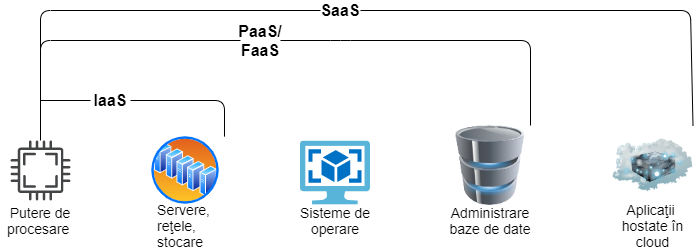
\includegraphics[width=1\textwidth]{images/cloudDiagram}
			 \caption{Componentele diverselor modele de procesare în cloud}
			 \label{fig:cloud_diagram}
\end{center}
\end{figure}
\\
Categoriile de servicii cloud sunt : 
\begin{itemize}
\item Infrastructure as a Service (IaaS)
\item Software as a Service (SaaS) 
\item Platform as a Service (PaaS) 
\item Function as a Service (FaaS) 
\end{itemize}
\par Soluţiile de tip \emph{IaaS} presupun punerea la dispoziţia clientului doar a infrastructurii cerute, fără nici o administrare din partea distribuitorului. Din acest punct de vedere, soluţiile IaaS pot fi vazute de către client drept infrastructuri fizice, singura diferenţă fiind că locul în care este amplasată aparatura nu este deţinută de către client. În ceea ce priveşte securitatea, update-urile, softurile şi toate legăturile din cadrul infrastructurii, acestea sunt administrate strict de către client. Între a rula un sistem pe o infrastructură locală şi a rula un sistem pe o infrastructura aflată in cloud dar folosind o soluţie IaaS există doar diferenţe de natură economică. 

\par \emph{SaaS} reprezintă o metodă pentru distribuirea softurilor pe internet la cerere şi pe bază de subscripţie. Soluţiile SaaS sunt folosite pentru găzduirea şi adminstrarea softurilor pentru a facilita distribuţia de update-uri sau pathcuri de securitate.

\par Soluţiile \emph{PaaS} reprezintă un mod de a crea medii de dezvoltare, testare sau producţie la cerere. Este construit pentru a asigura o modalitate rapidă de a crea aplicaţii software diverse, de la aplicaţii web, la cele mobile sau API-uri ce fac parte dintr-un alt sistem. Practic, este un mod de a creea si administra soluţii IaaS în mod automat, asigurând toate uneltele necesare pentru scalabilitate automată, distribuirea traficului între servere, mentenanţă, asigurarea securităţii şi lansarea de noi versiuni. Deşi este un serviciu serverfull, acesta ia de pe umerii clientului sarcina creeri şi administrării infrastructurii, grăbind astfel procesul de dezvoltare şi lansare a unui nou sistem software.

\par In ceea ce priveşte FaaS, acesta este un domeniu nou, deoarece a apărut pentru prima dată în 2010 fiind oferit de câteva start-upuri la acea vreme. Acest mod de dezvoltare orientat spre microservicii a devenit trendul in industrie în ultimii ani pentru sisteme cu potenţial de scalare mare, deoarece prezintă numeroase avantaje din punct de vedere al modului de dezvoltare şi de execuţie în industrie. În momentul de faţă, pentru servicii de tip FaaS sunt 3 mari jucători: Amazon cu AWS Lambda, Google cu Google Cloud Functions si Microsoft cu Azure Functions.\cite{jonas2019cloud}. Numeroase lucrări din domeniu \cite{christidis2019, wang2019} arată ca rularea algoritmilor de machine learning folosind soluţii FaaS (Function as a service) precum AWS Lambda sau Google cloud functions, este în sine o problemă ce necesită soluţii de optimizare a codului pentru a indeplini restricţiile soluţiilor de rulare serverless, cum ar fi memoria limitată a mediului de execuţie. 
\par 
O altă caracteristica a soluţiilor cloud este tipul de execuţie şi anume: \emph{serverfull} sau \emph{serverless}.
Prin serverfull, se inţelege o soluţie ce rulează pe servere ce pot fi indentificate în mod unic, care rulează în mod continuu, dar pe care se execută diferite operaţii în funcţie de nevoile sistemului. IaaS si PaaS sunt mereu soluţii serverfull, în timp ce un serviciu SaaS poate fi atât serverfull cât si serverless.
Prin serverless se inţelege o soluţie ce lansează noi micro-instanţe pentru fiecare cerere, ce este mai apoi oprită dupa execuţia codului. Costul unei soluţii serverless este direct proporţional cu timpul de execuţie, în timp ce pentru soluţiile serverfull costul este constant. \\
\clearpage
\par Caracteristicile celor 2 tipuri sunt prezentate în tabelul de mai jos :
\begin{table}[h]
\begin{tabular}{|l|l|l|}
\hline
Caracteristici             & Soluţii AWS serverless                  & Soluţii AWS serverfull                          \\ \hline
Când este activ serviciul & Când este declanşat de un eveniment     & Continuu, până la oprire \\ \hline
Limbaj de programare      & Python, Java, Go, C\#,  şi altele...    & Orice limbaj                                     \\ \hline
Max RAM                   & 0.125 - 3 Gb                            & 0.5-1952 Gb                                      \\ \hline
Max Capacitate de stocare & 0.5 Gb                                  & 0-3600 Gb                                        \\ \hline
Max Timp de rulare        & 900 secunde                             & Nelimitat                                        \\ \hline
Unitatea minimă taxată    & 0.1 secunde                             & 60 de secunde                                    \\ \hline
Preţ minim pe unitate     & \$0.0000002                             & \$0.0000867                                      \\ \hline
Sistem de operare         & Ales de distribuitorul de soluţii cloud & Ales de către client                             \\ \hline
\end{tabular}
\end{table}

\section{Comparaţie între soluţiile PaaS si FaaS}
\quad Atât soluţiile PaaS cât şi cele FaaS sunt pretabile sistemelor de inteligenţă artificială, deoarece oferă administrare automată, putere mare de calcul şi  avantajul că suportă optimizari prin rularea pe GPU.
\par Soluţiile PaaS, deşi oferă servicii de adminstrare automată, în spatele acestui mecanism se ascunde tot o infrastructură clasică, cu servere fizice ce rulează în mod continu, ce necesită echilibrarea traficului între acestea, lansarea de noi servere, lansarea de noi versiuni a aplicaţiei pe serverele deja pornite sau închiderea unor servere atunci cand nu mai sunt folosite. Toate acestea sunt realizate de către distribuitorul de soluţii cloud, punând la dispoziţia clientului un mediu gata să suporte orice tip de trafic către aplicaţie.  Astfel dezvoltatorul se poate gândi doar la construirea unui server cât mai eficient, pentru a folosi resursele unei instanţe la maxim. Un aspect important pentru soluţiile PaaS este costul asociat instanţelor folosite. Deşi numarul lor este variabil, în orice moment măcar o instanţa trebuie sa fie activă. Asta inseamnă că dacă sistemul poate rula doar pe instanţe cu resurse suplimentare, ce au un cost orar mai mare, sistemul va avea un cost de operare mare chiar şi atunci cand este subutilizat. Un sistem ce foloseşte soluţii PaaS în mod ideal este de preferat sa ruleze pe mai multe instanţe cu capacitate de execuţie mică faţă de mai puţine instanţe cu capacitate mare, deoarece lansarea sau inchiderea de noi instanţe este gratuită, în timp ce rularea acestora atunci când sunt sub-utilizate nu este.
\par Soluţiile FaaS, pe de alta parte, abstractizează si mai mult infratructura existentă, luând orice responsabilitate de pe umerii clienţilor atunci când vine vorba de adminstrarea acesteia. FaaS presupune existenţa unei funcţii, ce simbolizează o aplicaţie, ce este executată de fiecare dată când apare un eveniment declanşator. Avantajul acestei abordări este costul asociat, şi anume faptul ca plata se realizează strict pentru timpul în care funcţia a fost executată. Timpul petrecut pentru a aştepta apariţia unui eveniment nu este taxat. Spre exemplu, soluţia FaaS a celor de la Amazon, AWS Lambda, poate fi declanşată în numeroase moduri, de la încarcarea unui fişier într-o destinaţie S3 prestabilită, la un apel HTTP către un endpoint ataşat funcţiei. Aceste soluţii suportă majoritatea limbajelor de programare, şi pot fi configurate în aşa fel încat sa acopere orice nevoie în ceea ce priveşte puterea de execuţie.
Soluţiile FaaS prezintă şi o serie de dezavantaje printre care se numară:
\begin{itemize} 
\item Există o limită asupra dimensiunii codului ce urmează sa fie executat de către funcţie.
\item Timpul de execuţie a unei funcţii este deasemenea limitat.
\item Starea programului nu este pastrată între execuţii facând necesară stocarea datelor ce trebuie să persiste în locaţii dedicate (S3 sau o bază de date)
\item Limitarea executării concurente. (Lambda nu permite mai mult de 1000 de funcţii sa fie executate concomitent)
\end{itemize} 
\par Deşi din descrierea acestui tip de soluţii, pare alegerea ideală pentru execuţia etapei de inferenţă pentru un model de \emph{machine learning}, situaţia devine complicată atunci când sistemul este unul complex, iar respectarea acestei limite de dimensiune devine un blocaj. De multe ori, aplicaţiile de AI/ML depind de biblioteci si frameworkuri cunoscute în domeniu precum \emph{ tensorflow, keras, mxnet}, dar care au fost dezvoltate având în minte eficienţa execuţiei, şi nu minimizarea codului sursă. Având în vedere ca AWS Lambda limitează dimensiunea codului ataşat la 250MB, lansarea sistemelor ce se bazează pe reţele neuronale este o sarcină grea din punct de vedere al încadrării în aceste restricţii. 
\section{Descrierea soluţiei curente}
\quad Soluţia aleasă pentru execuţia etapei de inferenţă în cloud este \emph{AWS Elastic Beanstalk}. Acest serviciu de tip PaaS oferă mediul perfect pentru lansarea aplicaţiei, atât din punct de vedere al configurabilităţii cât şi al securităţii oferite. 
Pentru a lansa o aplicaţie folosind elastic beanstalk, este necesar să creezi un pachet de lansare, ce conţine codul sursă şi celelalte instrucţiuni pentru iniţializarea serviciului. Deşi acesta este limitat la 512MB, este mai mult decât indeajuns deoarece mediul de rulare si dependinţele programului nu sunt adaugate în acest pachet, ci sunt descarcate pe server la momentul lansării pe baza unui fişier de configurare adaugat în pachet numit \emph{requirements.txt}.\\
În timpul lansării aplicaţiei, sunt create automat următoarele resurse : 
\begin{itemize}
\item O flotă , sau o singură instanţă \emph{EC2}, în funcţie de configuraţie
\item Un \emph{Elastic Load Balancer} ce distribuie traficul între instanţe
\item Un \emph{AutoScaling Group} ce defineşte regulile de scalare a numărului de instanţe
\item O destinaţie \emph{S3} în care este stocat codul sursă al aplicaţiei
\item Şi un \emph{API Gateway} ce joacă rolul de punct de intrare al traficului în aplicaţie
\end{itemize}
\par Deoarece la bază se află instanţe EC2, acestea oferă un mare avantaj din punct de vedere al execuţiei concurente acestei soluţii faţă de AWS Lambda sau alte soluţii FaaS asemanătoare. Deşi mai multe instanţe Lambda pot fi executate concurent, în cadrul unei singure instanţe, apelurile concurente nu sunt permise. Luând în calcul că în etapa de inferenţă sunt şi părţi de input/output în care resursele sunt nefolosite, folosirea instanţelor EC2 ce pot rula mai multe apeluri în mod concurent este opţiunea optimă din punct de vedere al folosirii resurselor. 
\par Capacitatea de multi-threading din cadrul serverelor, la care se adaugă scalarea automată a numarului acestora în funcţie de traficul ce accesează API-ul, face ca resursele sa fie folosite la maxim, atât din punct de vedere al performanţei disponibile, cât şi din punct de vedere economic. 
\par Un alt avantaj al acestei soluţii este usurinţa cu care se poate schimba mediul de execuţie. Spre exemplu, într-un anumit scenariu, în care se observă în panoul de monitorizare că instanţele EC2 curente sunt suprasolicitate, cu ajutorul interfeţei web, sau celei din linia de comandă, pot fi schimbate tipurile de instanţe EC2 folosite cu unele mai performante fără a avea serviciul indisponibil pe durata acestei modificări.

\chapter {Rezultate şi Concluzii}

\quad Sistemul a fost evaluat pe setul de date \emph{Avenue} . Ca şi modalitate de evaluare a fost luată în considerare aria de sub curbă (eng: \emph {area under the curve (AUC)}) raportată la scorul fiecărui cadru. 
\par Scorul unui cadru reprezintă maximul dintre scorurile obţinute de obiectele din imagine. Această valoare este valoroasă şi în practică, deoarece pe baza acesteia se pot izola cadrele ce au un scor de anomalie peste un anumit nivel. Pentru a evalua întregul set de date, au fost evaluate individual video-urile de test, iar mai apoi a fost calculată media scorurilor obţinute, metodă folosită şi de către  \emph{Ionescu et al.} \cite{ionescu2019object}.
\par 
\begin{wrapfigure}{r}{0.45\textwidth}
\begin{center}
        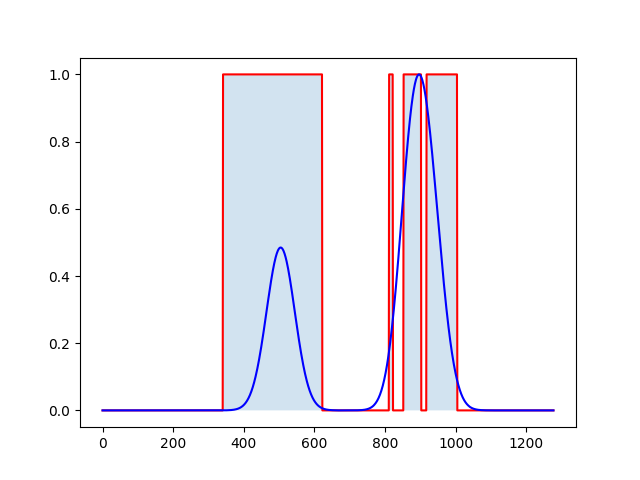
\includegraphics[width = 0.5\textwidth]{images/rezultate_video_6}
			 \caption{Scorurile la nivel de cadru pentru video-ul nr.6 din setul de date Avenue. Scorul fiecărui cadru este marcat cu albastru închis, în timp ce zonele cu fundal albastru deschis reprezintă perioadele în care au existat anomalii.}
			 \label{fig:results_6}
\end{center}
\end{wrapfigure}
\quad Rezultatele sistemului sunt de (65 \%), sub cele prezentate în lucrarea iniţiala  \cite{ionescu2019object}, datorate orientării spre viteză pe sisteme ce nu posedă GPU, limitărilor fizice ale maşinii folosite pentru antrenare şi a folosirii unei librării diferite pentru etapa de inferenţă.
\par Aşa cum se observă şi în figura ~\ref{fig:results_6} sistemul izolează cu succes evenimentele anormale. Totuşi, detecţia obiectelor rămâne cel mai mare dezavantaj al sistemului, deoarece, atât din punct de vedere al timpului de execuţie, cât şi al performanţei, acesta este locul în care sistemul poate fi imbunătăţit. Faţă de sistemul de referinţă  \cite{ionescu2019object}, alegerea unui nou tip de detector de obiecte optimizat pentru execuţia pe CPU, a crescut viteza de la 0.8 FPS la 8 FPS pe sisteme ce nu posedă GPU, ceea ce reprezintă o îmbunătăţire semnificativă a sistemului. Însă, deşi mai rapid, noul detector nu realizează operaţia de segmentare la fel de bine pentru obiectele mici, sau îndepărtate de cameră lucru ce face ca pe setul de date Avenue, să nu obţine performanţe la fel de bune ca sistemul iniţial. 
\par Majoritatea detecţiilor fals pozitive ale sistemului sunt în mare parte cauzate de segmentarea imperfectă a detectorului de obiecte(fig.  ~\ref{fig:eroare_detectie}). În urma experimentelor a reieşit ca situaţiile în care mai multe se află în acelaşi cadran, sau 1 obiect nu este încadrat complet de către cadran pun probleme sistemului şi generează detecţii fals pozitive. În următoarele versiuni ale ale sistemului se vor încerca modalităţi de filtrare şi validare a detecţiilor de obiecte, pentru a elimina aceste probleme. 
\begin{figure}[h]
\begin{center}
        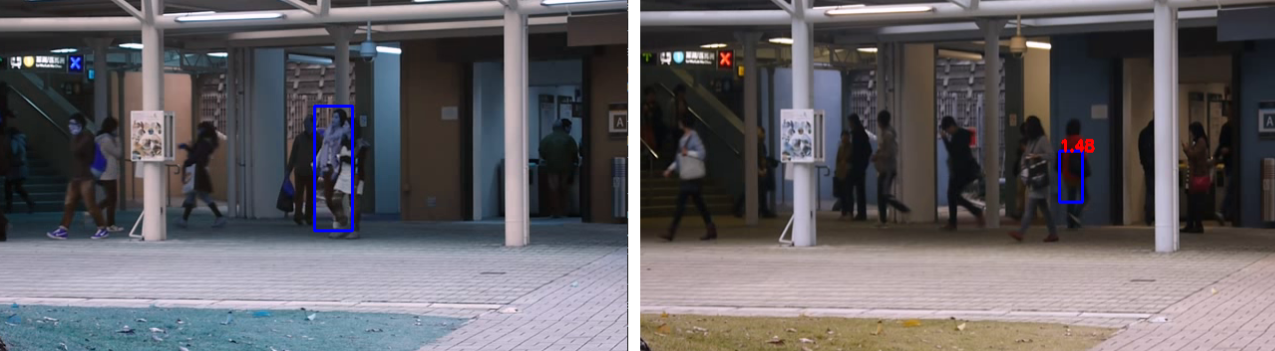
\includegraphics[width = 1\textwidth]{images/eroare_detectie}
			 \caption{Detecţii fals pozitive datorate detecţiei deficitare a marginilor obiectelor de către detectorul de obiecte. În prima imagine se poate observa un cadran ce conţine 2 persoane, în timp ce in cea de a 2-a imagine, cadranul ce ar fi trebuit să încadreze persoana în totalitate, conţine doar o mică parte din aceasta.}
			 \label{fig:eroare_detectie}
\end{center}
\end{figure}
\par Pentru a demonstra capacităţile sistemului de a detecta anomalii în absenţa erorilor de detecţie a obiectelor, am înregistrat un nou set de date, ce conţine persoane în plan apropiat, simulând o sală de aşteptare de capacitate redusă (e.g. cabinet dentar, secretariat, clinica de dimensiune redusă, etc.). Acest set de date conţine 4 videouri de antrenament ce reprezintă comportamentul normal al subiecţilor, şi 4 video-uri de test în care sunt exemplificate diverse comportamente anormale, precum :
\begin{itemize}
\item Alergare
\item Confruntări
\item Leşin
\item Vandalism 
\end{itemize}
\par Rezultatele empirice obţinute pe acest set de date, sunt satisfăcătoare, fiind detectate toate evenimentele anormale. 
\section {Timpi de execuţie şi necesarul de resurse}
\quad Din punct de vedere al timpului de execuţie al întregului sistem, acesta necesită 130 de milisecunde, din care 120 de milisecunde sunt petrecute detectând obiecte, şi 10 milisecunde trecând obiectele prin encoder şi apoi prin clasificatorul final. Astfel, sistemul evaluează cadrele cu o viteză de  8 cadre pe secundă. În ceea ce priveşte accesarea API-ului, sunt necesare în medie 1.1 secunde pentru încărcarea imaginilor ce vor fi procesate în cloud, şi 0.7 secunde pentru execuţia apelului HTTP propriu zis.
\begin{figure}[h]
\begin{center}
        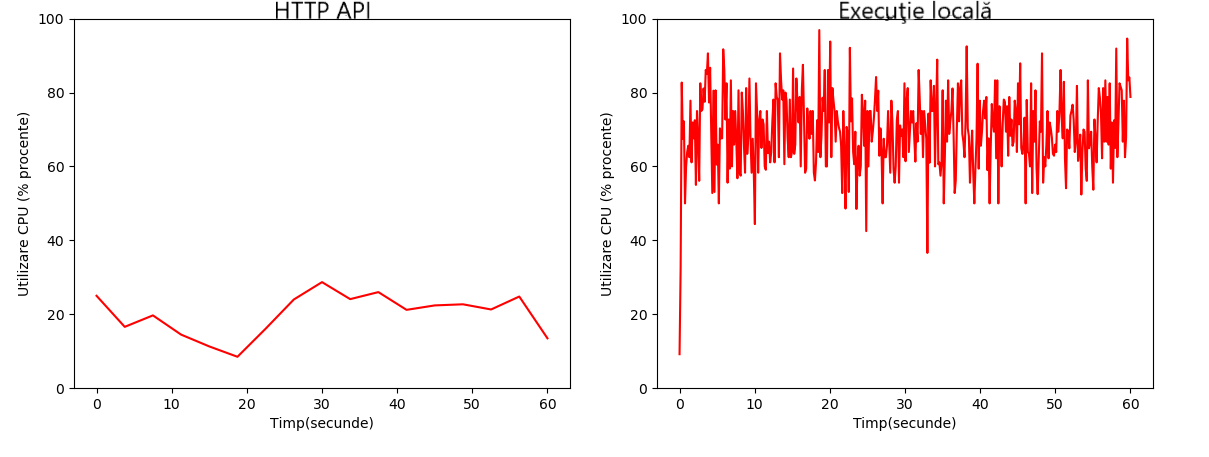
\includegraphics[width = 1\textwidth]{images/comparatie_cpu_usage}
			 \caption{Comparaţie între resursele folosite în timpul execuţiei sistemului timp de 1 minut, execuţie locală versus folosind API-ul.}
			 \label{fig:comparatie_cpu}
\end{center}
\end{figure}
\par Din punct de vedere al necesarului de resurse, am comparat cele 2 moduri de utilizare a sistemului : prin rulare locală, sau prin accesarea HTTP API-ului. 
Rezultatele prezentate in figura ~\ref{fig:comparatie_cpu} demonstrează economia de resurse făcută accesând API-ul. Astfel, sistemul poate fi folosit în 2 moduri : 
\begin{itemize}
\item Rapid dar ce foloseşte intens procesorul sistemului. În acest mod se pot rula şi analize în timp real.
\item Lent dar cu un necesar foarte scăzut de resurse. Acest mod poate fi folosit atunci când viteza de analiză nu este importantă.
\end{itemize}
\par Menţionez ca toate măsurătorile au fost realizate pe un sistem cu i7-6600U 2.6 GHz CPU şi 16 GB RAM.

\section{Concluzii}
\quad Sistemul de detectare a anomaliilor dezvoltat a îndeplinit asteptările iniţiale, îmbunătăţind viteza pe sisteme ce posedă resurse limitate. De asemenea, a fost creat un cadru ce face posibilă convertirea sistemelor clasice de supraveghere în sisteme inteligente, prin rularea sistemului de detecţie a anomaliilor fie local, fie prin intermediul arhitecturii client-server. 
\parÎn versiunile viitoare, se propune îmbunătăţirea preciziei sistemului, menţinând viteza curentă de execuţie. 
\bibliographystyle{abbrv}
\listoffigures
\listoftables
\bibliography{References}
\end{document}